%%%%%%%%%%%%%%%%%%%%%%%%%%%%%%%%%%%%%%%%%
% Masters/Doctoral Thesis 
% LaTeX Template
% Version 2.3 (25/3/16)
%
% This template has been downloaded from:
% http://www.LaTeXTemplates.com
%
% Version 2.x major modifications by:
% Vel (vel@latextemplates.com)
%
% This template is based on a template by:
% Steve Gunn (http://users.ecs.soton.ac.uk/srg/softwaretools/document/templates/)
% Sunil Patel (http://www.sunilpatel.co.uk/thesis-template/)
%
% Template license:
% CC BY-NC-SA 3.0 (http://creativecommons.org/licenses/by-nc-sa/3.0/)
%
%%%%%%%%%%%%%%%%%%%%%%%%%%%%%%%%%%%%%%%%%

%----------------------------------------------------------------------------------------
%	PACKAGES AND OTHER DOCUMENT CONFIGURATIONS
%----------------------------------------------------------------------------------------

\documentclass[
11pt, % The default document font size, options: 10pt, 11pt, 12pt
%oneside, % Two side (alternating margins) for binding by default, uncomment to switch to one side
%chapterinoneline,% Have the chapter title next to the number in one single line
%english, % ngerman for German
spanish,
singlespacing, % Single line spacing, alternatives: onehalfspacing or doublespacing
%draft, % Uncomment to enable draft mode (no pictures, no links, overfull hboxes indicated)
%nolistspacing, % If the document is onehalfspacing or doublespacing, uncomment this to set spacing in lists to single
%liststotoc, % Uncomment to add the list of figures/tables/etc to the table of contents
%toctotoc, % Uncomment to add the main table of contents to the table of contents
parskip, % Uncomment to add space between paragraphs
%nohyperref, % Uncomment to not load the hyperref package
headsepline, % Uncomment to get a line under the header
]{MastersDoctoralThesis} % The class file specifying the document structure



\usepackage[utf8]{inputenc} % Required for inputting international characters
\usepackage[T1]{fontenc} % Output font encoding for international characters

\usepackage{palatino} % Use the Palatino font by default
%,style=authoryear
\usepackage[backend=bibtex,natbib=true]{biblatex} % Use the bibtex backend with the authoryear citation style (which resembles APA)

\addbibresource{references.bib} % The filename of the bibliography

\usepackage[autostyle=true]{csquotes} % Required to generate language-dependent quotes in the bibliography

\usepackage{caption}
\usepackage{subcaption}

%------------------------
\usepackage{listings}

%\usepackage[hyphens]{url}
%\usepackage[hidelinks]{hyperref}
%\hypersetup{breaklinks=true}
\urlstyle{same}
%\usepackage{cite}

%--------------------------

\usepackage{color}

%
%----------------------------------------------------------------------------------------
%	MARGIN SETTINGS
%----------------------------------------------------------------------------------------

\geometry{
	paper=a4paper, % Change to letterpaper for US letter
	inner=2cm, % Inner margin
	outer=3.3cm, % Outer margin
	bindingoffset=2cm, % Binding offset
	top=1.5cm, % Top margin
	bottom=1.5cm, % Bottom margin
	%showframe,% show how the type block is set on the page
}

%----------------------------------------------------------------------------------------
%	INFORMACIÓN DE LA MEMORIA
%----------------------------------------------------------------------------------------

\thesistitle{Medidor de energía eléctrica industrial con telemetría} % El títulos de la memoria, se usa en la carátula y se puede usar el cualquier lugar del documento con el comando \ttitle
\supervisor{Esp. Ing. Nicolás Álvarez} % El nombre del director, se usa en la carátula y se puede usar el cualquier lugar del documento con el comando \supname
\degree{Especialista en Sistemas Embebidos } % Nombre del grado, se usa en la carátula y se puede usar el cualquier lugar del documento con el comando \degreename
\author{Hernán Darío Ferreyra} % Tu nombre, se usa en la carátula y se puede usar el cualquier lugar del documento con el comando \authorname
\juradoUNO{Sr. Juan Manuel Cruz Beaufrere (pertenencia)} % Nombre y pertenencia del un jurado se usa en la carátula y se puede usar el cualquier lugar del documento con el comando \jur1name
\juradoDOS{Dr. Mariano García Inza (pertenencia)} % Nombre y pertenencia del un jurado se usa en la carátula y se puede usar el cualquier lugar del documento con el comando \jur2name
\juradoTRES{Esp. Ing. Sergio Renato De Jesús Meleán (pertenencia)} % Nombre y pertenencia del un jurado se usa en la carátula y se puede usar el cualquier lugar del documento con el comando \jur3name
\fechaINICIO{Agosto de 2018}
\fechaFINAL{Diciembre de 2019}

\subject{Memoria del Trabajo Final de la Carrera de Especialización en Sistemas Embebidos de la UBA} % Your subject area, this is not currently used anywhere in the template, print it elsewhere with \subjectname
\keywords{CESE, Sistemas Embebidos, CIAA} % Keywords for your thesis, this is not currently used anywhere in the template, print it elsewhere with \keywordnames
\university{Universidad de Buenos Aires} % Your university's name and URL, this is used in the title page and abstract, print it elsewhere with \univname
\faculty{{Facultad de Ingeniería}} % Your faculty's name and URL, this is used in the title page and abstract, print it elsewhere with \facname
\department{Departamento de Electrónica} % Your department's name and URL, this is used in the title page and abstract, print it elsewhere with \deptname
\group{{Laboratorio de Sistemas Embebidos}} % Your research group's name and URL, this is used in the title page, print it elsewhere with \groupname


\hypersetup{pdftitle=\ttitle} % Set the PDF's title to your title
\hypersetup{pdfauthor=\authorname} % Set the PDF's author to your name
\hypersetup{pdfkeywords=\keywordnames} % Set the PDF's keywords to your keywords


\newcaptionname{spanish}{\acknowledgementname}{Agradecimientos}
\newcaptionname{spanish}{\authorshipname}{Declaración de Autoría}
\newcaptionname{spanish}{\abbrevname}{Glosario}
\newcaptionname{spanish}{\byname}{por}

\renewcommand{\lstlistingname}{Algoritmo}% Listing -> Algorithm
\renewcommand{\lstlistlistingname}{Índice de \lstlistingname s}% List of Listings -> List of Algorithms

\renewcommand{\listtablename}{Índice de Tablas}
\renewcommand{\tablename}{Tabla} 

\addtolength{\footnotesep}{2mm} % Espacio adicional en los footnotes

\begin{document}

\frontmatter % Use roman page numbering style (i, ii, iii, iv...) for the pre-content pages

\pagestyle{plain} % Default to the plain heading style until the thesis style is called for the body content

%----------------------------------------------------------------------------------------
%	CARÁTULA
%----------------------------------------------------------------------------------------

\begin{titlepage}
\begin{center}

{\scshape\LARGE UNIVERSIDAD DE BUENOS AIRES\par}\vspace{0.1cm} % University name
{\scshape\LARGE FACULTAD DE INGENIERÍA\par}\vspace{0.1cm} % Faculty name
{\scshape\LARGE Carrera de Especialización en Sistemas Embebidos\par}\vspace{1cm} % Thesis type


\includegraphics[width=.3\textwidth]{./Figures/logoFIUBA.png}
\vspace{1cm}

\textsc{\Large Memoria del Trabajo Final}\\[0.5cm] % Thesis type

{\huge \bfseries \ttitle\par}\vspace{0.4cm} % Thesis title

\vspace{1cm}
\LARGE\textbf{Autor:\\
\authorname}\\ % Author name

\vspace{1cm}

\large
\vspace{10px}
{Director:} \\
{\supname} % Supervisor name
 
\vspace{1cm}
Jurados:\\
\jurunoname\\
\jurdosname\\
\jurtresname
 
\vfill
\textit{Este trabajo fue realizado en las Ciudad Autónoma de Buenos Aires, entre \fechaINICIOname \hspace{1px} y \fechaFINALname.}
\end{center}
\end{titlepage}


%----------------------------------------------------------------------------------------
%	RESUMEN - ABSTRACT 
%----------------------------------------------------------------------------------------

\begin{abstract}
\addchaptertocentry{\abstractname} % Add the abstract to the table of contents
%
%The Thesis Abstract is written here (and usually kept to just this page). The page is kept centered vertically so can expand into the blank space above the title too\ldots
\centering
Este trabajo presenta el desarrollo de un prototipo de hardware y de su respectivo firmware. El prototipo es capaz de realizar la medición de tensión alterna,  corriente alterna y potencia de una máquina o tablero eléctrico, proveyendo los valores medidos mediante diferentes salidas de si mismo. Además el dispositivo es capaz de realizar un corte de energía en caso de alarma por tensión o corriente y de almacenar datos.
\end{abstract}

%----------------------------------------------------------------------------------------
%	CONTENIDO DE LA MEMORIA  - AGRADECIMIENTOS
%----------------------------------------------------------------------------------------

\begin{acknowledgements}
%\addchaptertocentry{\acknowledgementname} % Descomentando esta línea se puede agregar los agradecimientos al índice
\vspace{1.5cm}

Agradecimientos personales. \textbf{[OPCIONAL]} 

No olvidarse de agradecer al tutor.

No vale poner anti-agradecimientos (este trabajo fue posible a pesar de...)

\end{acknowledgements}

%----------------------------------------------------------------------------------------
%	LISTA DE CONTENIDOS/FIGURAS/TABLAS
%----------------------------------------------------------------------------------------
\renewcommand{\listtablename}{Índice de Tablas}

\tableofcontents % Prints the main table of contents

\listoffigures % Prints the list of figures

\listoftables % Prints the list of tables


%----------------------------------------------------------------------------------------
%	CONTENIDO DE LA MEMORIA  - DEDICATORIA
%----------------------------------------------------------------------------------------

\dedicatory{\textbf{Dedicado a... [OPCIONAL]}}  % escribir acá si se desea una dedicatoria

%----------------------------------------------------------------------------------------
%	CONTENIDO DE LA MEMORIA  - CAPÍTULOS
%----------------------------------------------------------------------------------------

\mainmatter % Begin numeric (1,2,3...) page numbering

\pagestyle{thesis} % Return the page headers back to the "thesis" style

\renewcommand{\tablename}{Tabla} 

% Incluir los capítulos como archivos separados desde la carpeta Chapters
% Descomentar las líneas a medida que se escriben los capítulos

% Chapter 1

\chapter{Introducción General} % Main chapter title

\label{Chapter1} % For referencing the chapter elsewhere, use \ref{Chapter1} 
\label{IntroGeneral}

%----------------------------------------------------------------------------------------

% Define some commands to keep the formatting separated from the content 
\newcommand{\keyword}[1]{\textbf{#1}}
\newcommand{\tabhead}[1]{\textbf{#1}}
\newcommand{\code}[1]{\texttt{#1}}
\newcommand{\file}[1]{\texttt{\bfseries#1}}
\newcommand{\option}[1]{\texttt{\itshape#1}}
\newcommand{\grados}{$^{\circ}$}

%----------------------------------------------------------------------------------------

%\section{Introducción}

%----------------------------------------------------------------------------------------
\section{Descripción general del trabajo y conceptos claves}

El trabajo desarrollado consiste en un sistema adquisidor de datos con los sensores necesarios para una medición de potencia eléctrica, en otras palabras un medidor digital de energía eléctrica. El trabajo fue desarrollado para una empresa privada localizada en Argentina.

Las mediciones eléctricas son los métodos, dispositivos y cálculos usados para medir cantidades eléctricas. La medición de cantidades eléctricas puede hacerse al medir parámetros eléctricos de un sistema. Usando transductores, propiedades físicas como la temperatura, presión, flujo, fuerza, y muchas otras pueden convertirse en señales eléctricas, que pueden ser convenientemente registradas y medidas. 

%\citep{MEcitation}

La adquisición de datos o adquisición de señales consiste en la toma de muestras del mundo real (sistema analógico) para generar datos que puedan ser manipulados por un ordenador u otros dispositivos electrónicos (sistema digital). Se requiere una etapa de acondicionamiento, que adecua la señal a niveles compatibles con el elemento que hace la transformación a señal digital.\cite{NIDataAdquisition}

\begin{figure}[h]
	\centering
	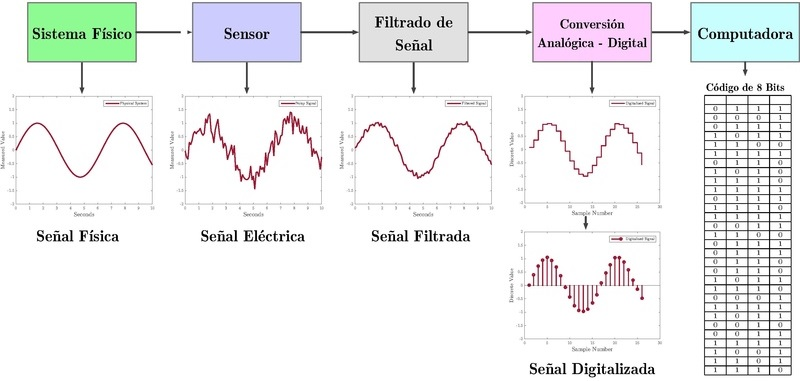
\includegraphics[width=120mm,keepaspectratio]{Figures/DigitalDAQ.jpg}
	\caption{Ejemplo de digitalización de una señal.}
	\label{fig:texmaker}
\end{figure}

Un convertidor de señal analógica a digital (ADC) es un dispositivo electrónico capaz de convertir una señal analógica, ya sea de tensión o corriente, en una señal digital mediante un cuantificador y codificándose en muchos casos en un código binario en particular. 
%\citep{ADCcitation}

\subsection{Sistemas electrónicos para mediciones eléctricas}

Las aplicaciones mas tempranas de computadores digitales a problemas de sistemas de potencia datan alrededor de 1940. La mayoría de las aplicaciones tempranas estaban limitadas en alcance debido a la pequeña capacidad de las tarjetas calculadoras usadas en ese periodo. Computadoras digitales de larga escalas estuvieron disponibles a mediados de 1950, y el éxito inicial de programas de flujo de carga llevaron al desarrollo de programas para cálculos de corto circuitos y estabilidad.\citep{761852}

Los medidores electrónicos digitalizan las variables medidas vía un ADC sigma delta  de alta resolución. La técnica de diseño de estos medidores digitales es influenciada por tres grandes factores: el costo , eficiencia y tamaño. Mientras que el costo esta influenciado por la capacidad de compra del cliente, la eficiencia y el tamaño deben cumplir estrictamente con los estándares.\cite{articleDM}

\begin{figure}[h]
	\centering
	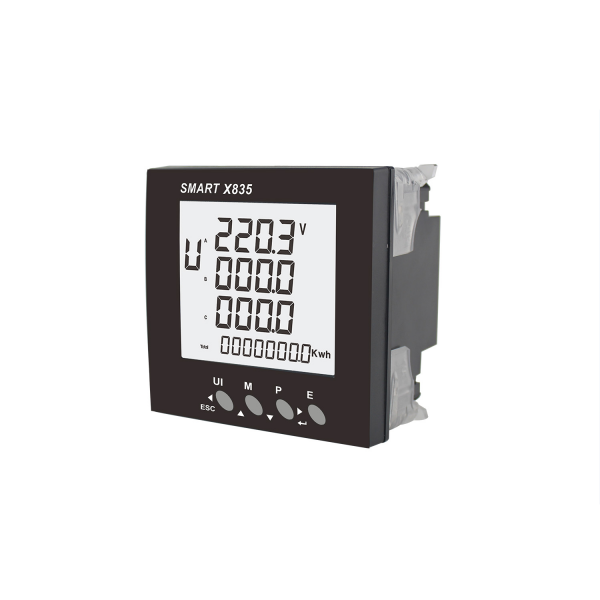
\includegraphics[width=55mm,keepaspectratio]{Figures/3931_1.png}
	\caption{Medidor electrónico comercial.}
	\label{fig:texmaker}
\end{figure}

La exactitud del medidor eléctrico digital depende en la exactitud del circuito analógico de entrada analógica, la exactitud del conversor analógico-digital y la exactitud de los cálculos digitales.\citep{Hribik2004DigitalPA}

Los convertidores analógicos-digitales basados en la modulación sigma - delta son económicamente viables para convertidores de alta resolución (mayores que 12bits), por lo que son  usados en el circuito integrado de procesadores de señales.

La modulación sigma-delta fue introducida en 1962 y no ganaría importancia hasta recientes desarrollos en tecnologías VLSI(integración a escala muy grande) que proveían fines prácticos para implementar complejos circuitos de procesamiento de señales.\citep{book:28601}


%%

\section{Motivación}

En la actualidad se pueden encontrar en el mercado internacional múltiples módulos electrónicos, de bajo costo, con puertos de comunicación para la medición de energía eléctrica como así también medidores digitales de energía de diferentes marcas para diferentes entornos, los que nos permite pensar que un dispositivo similar podría ser fabricado en la Argentina.

\begin{figure}[h]
	\centering
	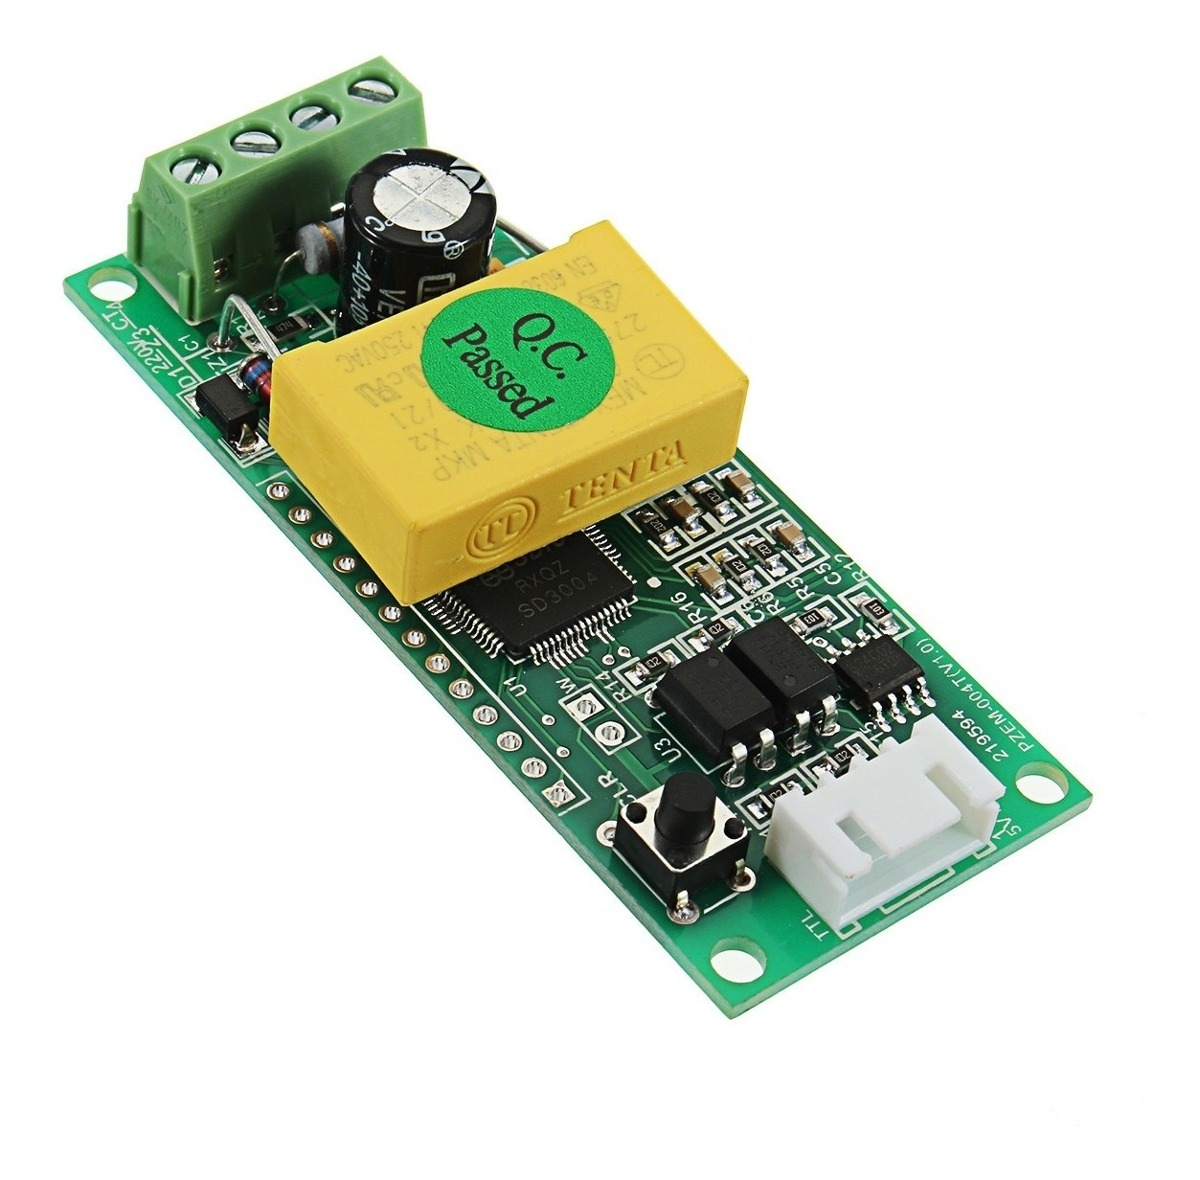
\includegraphics[width=80mm,keepaspectratio]{Figures/pzeem004.jpg}
	\caption{Modulo de medición de energía eléctrica con comunicación serie universal.}
	\label{fig:pzem04}
\end{figure}

Los módulos de medición pueden servir como un monitoreo de primera instancia pudiendo ser un método preventivo de fallas, dado que los parámetros de consumo dan una idea de estado de las máquinas.  El módulo de la figura \ref{fig:pzem04}  anterior fue usado en un trabajo de grado para un local comercial cuyo resultados pueden verse en la figura \ref{fig:graficoW}.  Estas gráficas sirvieron para realizar observaciones como el encendido de un motor trifásico y mal-funcionamiento de equipos de refrigeración.

\begin{figure}[h]
	\centering
	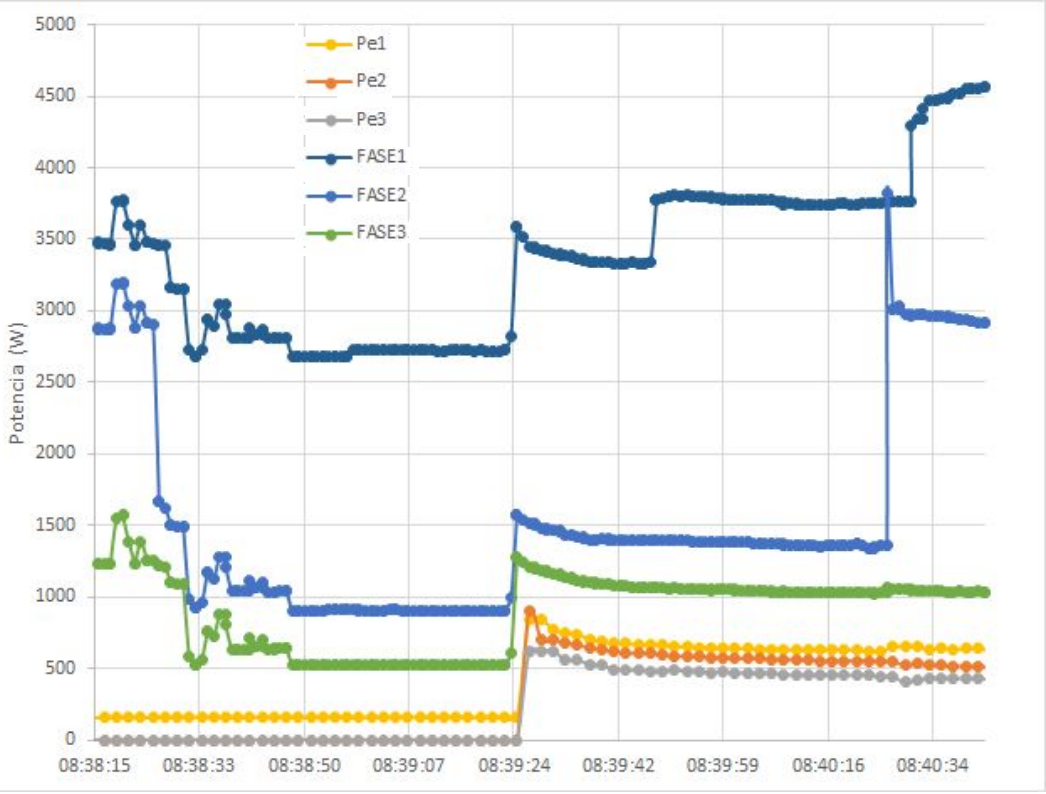
\includegraphics[width=80mm,keepaspectratio]{Figures/potencia_ej.png}
	\caption{Gráfico de medición de potencia mostrando el encendido de un frigorífico.}
	\label{fig:graficoW}
\end{figure}

Estos módulos se consiguen en el mercado internacional de modo que hay que importarlos lo que presenta una barrera para una herramienta de monitoreo simple. 

Desde el punto de vista de la empresa privada  el trabajo se planteó ante la necesidad de cuantificar consumos energéticos de procesos industriales para supervisar la alimentación de equipos de control o de medición. También como una alternativa a un producto anterior que solo media consumos de corriente continua. 

Por lo que la necesidad de hacer uso de la herramienta y la capacidad de realizar la electrónica de manera local  fueron los impulsores del trabajo realizado.

\section{Objetivos y alcance}

\subsection{Objetivos del desarrollo}
El objetivo del proyecto es el desarrollo de un dispositivo de medición, basado en un un micro-controlador de la familia MSP430 en conjunto con un ADC SOC(system on chip). Se pretende lograr un dispositivo comercial similar a aquellos elaborados anteriormente por la empresa privada, por lo que las dimensiones del PCB (printed circuit board) deberán ajustarse a los utilizados por las carcasas estándar que utiliza la empresa, como puede verse en la figura \ref{fig:disp_emp}.

\begin{figure}[h]
	\centering
	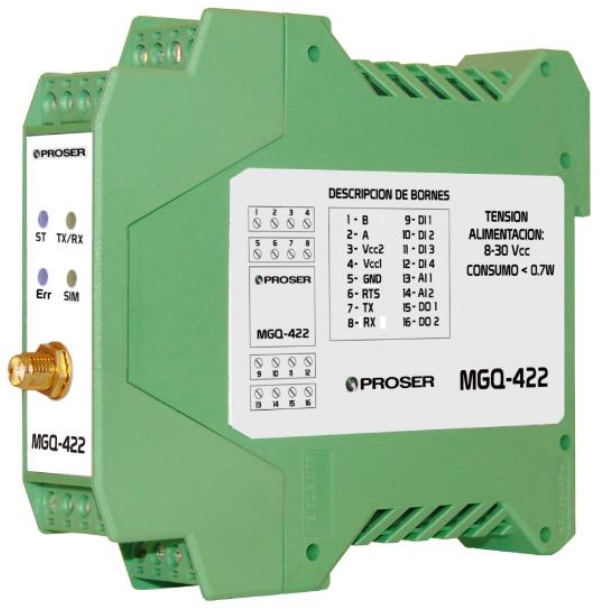
\includegraphics[width=80mm,keepaspectratio]{Figures/dispositivo_empresa.png}
	\caption{Ejemplo de dispositivo fabricado por la empresa privada.}
	\label{fig:disp_emp}
\end{figure}

Además se espera que el firmware maneje protocolo modbus y comunique las variables medidas a través de los puertos de comunicación. Físicamente se espera que el dispositivo sea capaz de comunicar por puertos serie RS-232 y RS-485, y ser diseñado pensando en su uso industrial (el dispositivo deberá ser robusto).


\subsection{Alcances}


%----------------------------------------------------------------------------------------

El trabajo abarca desde el planteo, diseño y fabricación de un pcb, la selección de componentes la elaboración del esquemático de conexiones lógicas, elaboración del pcb y su diseño teniendo en cuenta la fabricación de este hasta inclusive la elaboración de un prototipo y testeo sobre este.

También se espera que se  realice un firmware para el funcionamiento del dispositivo, teniendo en cuenta que el software debe incluir métodos de configuración para un futuro usuario.






\chapter{Introducción Específica} % Main chapter title

\label{Chapter2}

%----------------------------------------------------------------------------------------
%	SECTION 1
%----------------------------------------------------------------------------------------
En este capítulo se realiza una descripción del planeamiento y estructura del trabajo, sus requerimientos y características principales.

\section{Estructura del trabajo}
\label{sec:cap2parte1}
Inicialmente se realizó un plan de trabajo donde se plantea cómo se afronta el problema y el modo en que se lo resolverá. El proyecto consta de dos partes principales: hardware y software.

Para el hardware se planteó un diagrama de bloques que sirvió de guía al realizar el esquemático, que puede verse en la figura \ref{fig:bloquess1}. El diagrama plantea dos sectores uno de procesamiento y otro de medición que se encontraran aislados.

\begin{figure}[h]
	\centering
	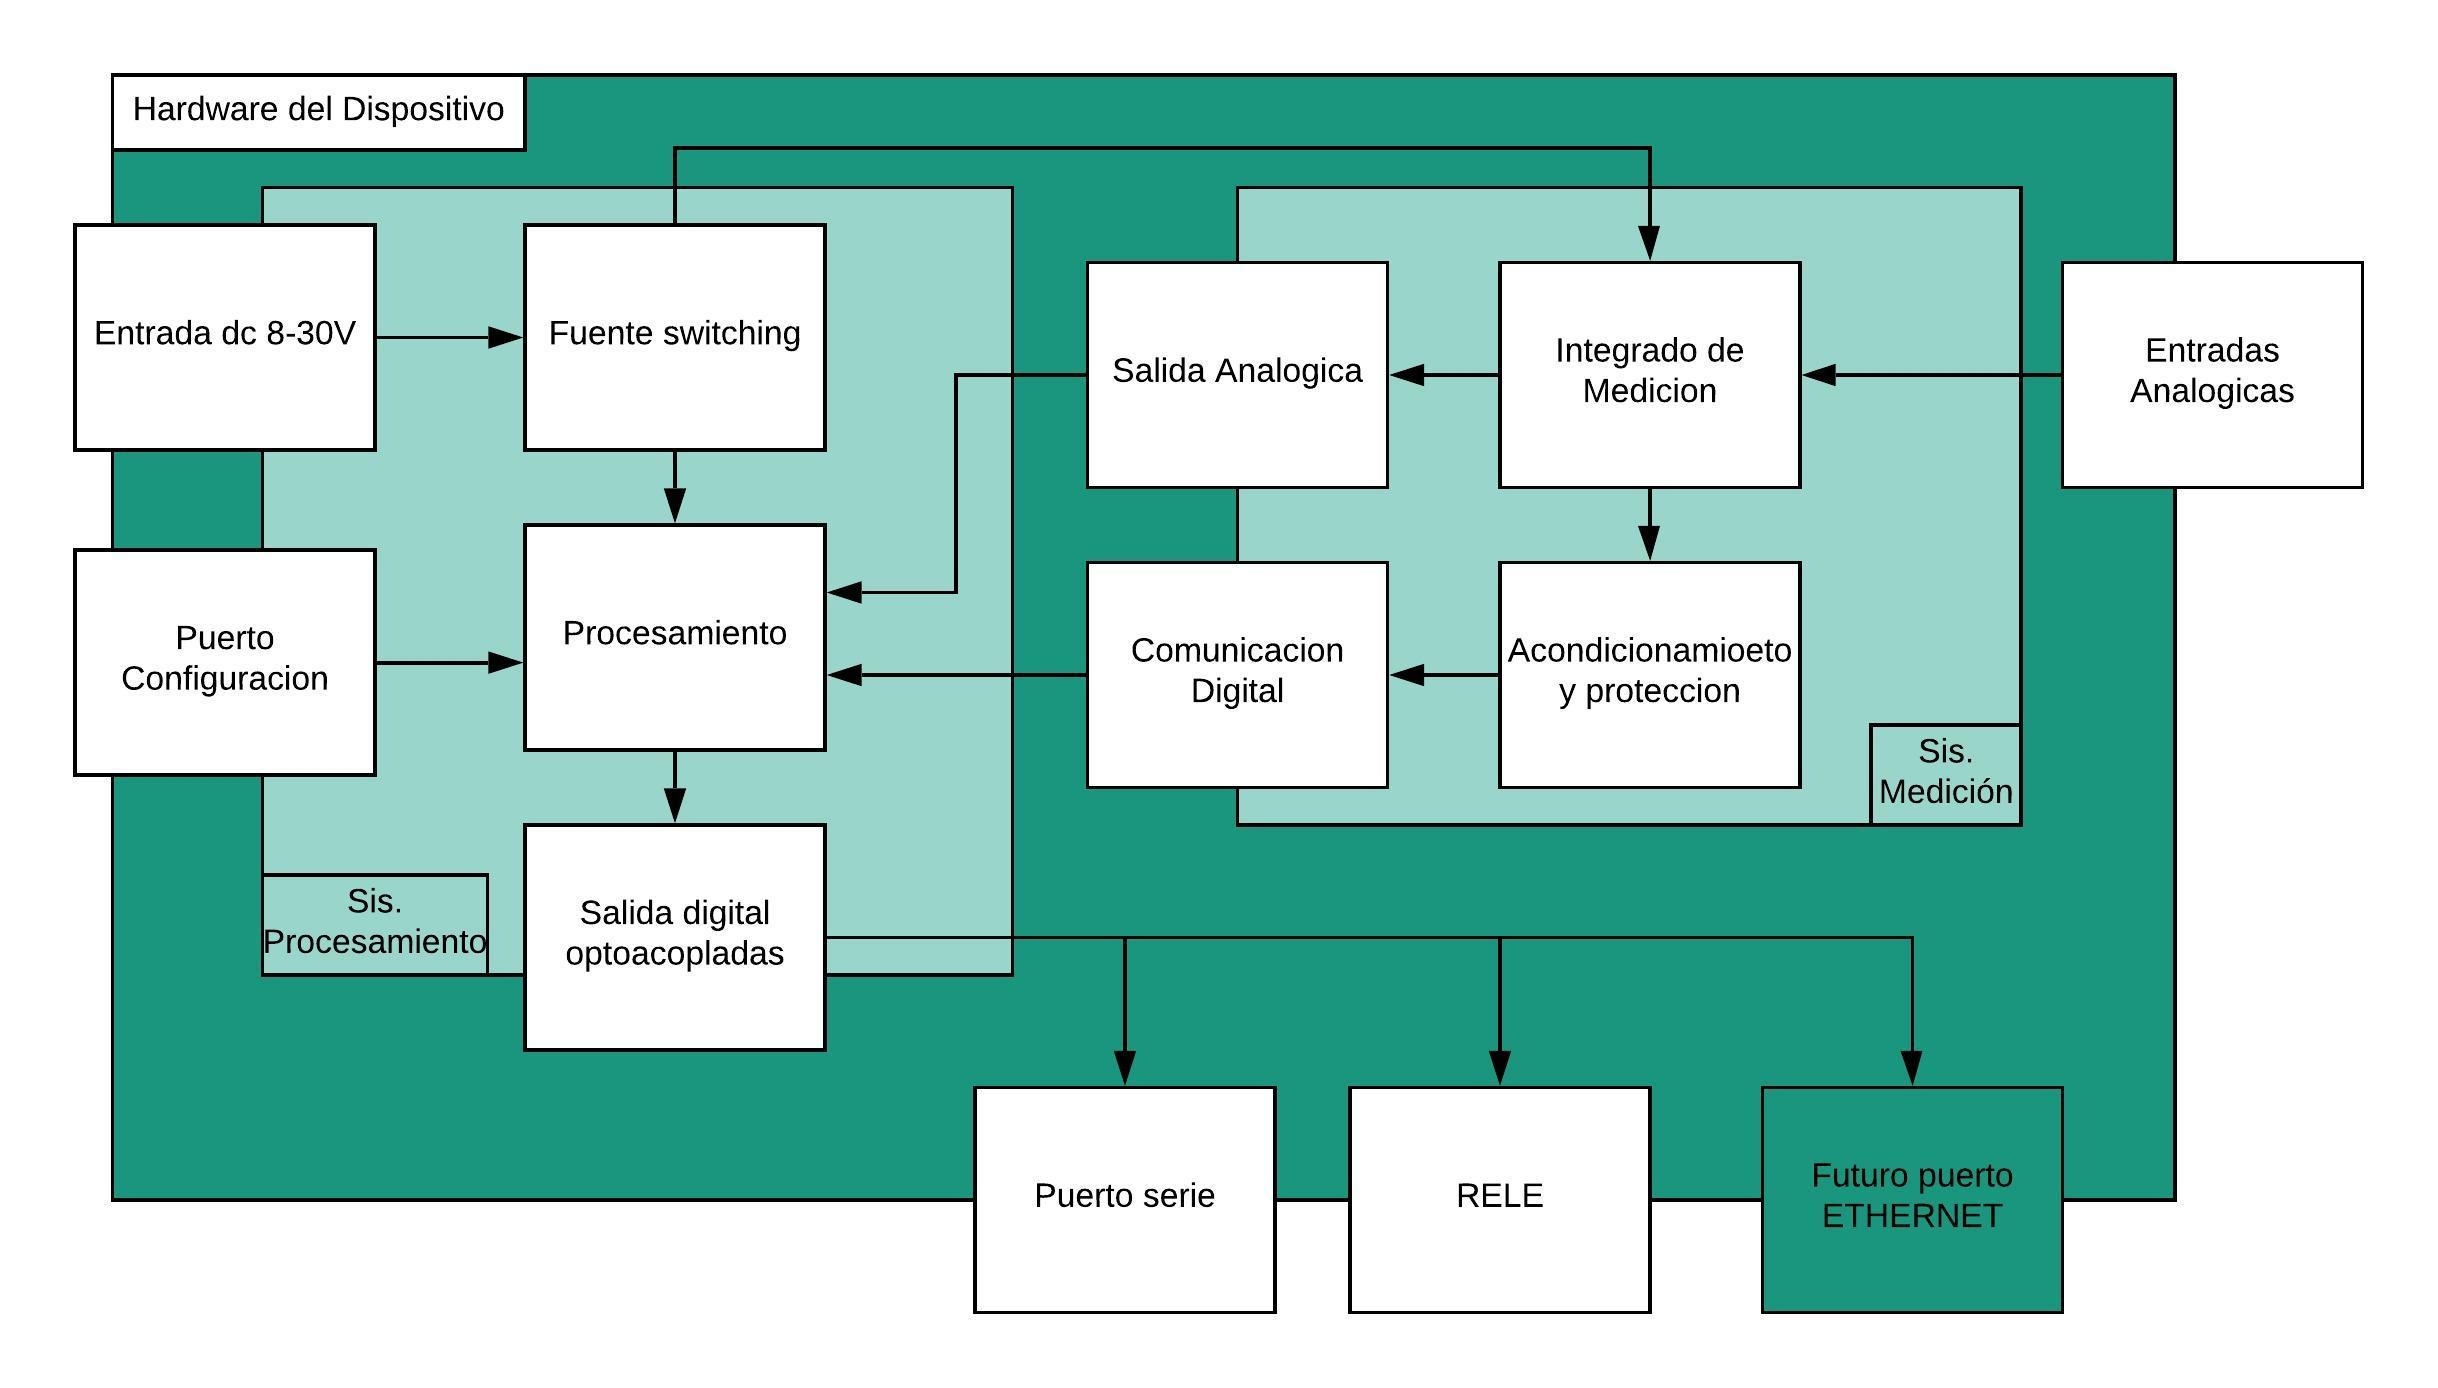
\includegraphics[width=120mm,keepaspectratio]{Figures/concepto.jpeg}
	\caption{Diagrama planteado para la elaboración de hardware.}
	\label{fig:bloquess1}
\end{figure}

El diagrama presupone que se usará una entrada de alimentación de corriente continua de 8 a 30 V conectado a una una fuente \textit{switching}, alimentando tanto al procesamiento como a la medición.

Del sistema de procesamiento se tiene que el hardware contara con un puerto de configuración y varias salidas optoacopladas, se plantea que estas salidas sean un relé ,un puerto serie y un puerto ethernet.

Del sistema de medición se observa comunicar al procesamiento por una comunicación digital aislada y también por una salida analógica. También se indica que la medición tendrá varias entradas analógicas, pero estas no fueron especificadas.

En cuanto el software se estableció que sea el necesario para lograr el testeo de las partes del hardware y la verificación de los requerimientos, por lo que el software debía manejar correctamente todos los integrados que fueran a estar embebidos en el circuito del dispositivo y manejar todos los protocolos definidos en los requisitos.

El enfoque inicial del trabajo fue el armado de la electrónica del prototipo, y el software se constituyó como la segunda parte que debía demostrar el correcto funcionamiento del hardware.

\section{Requerimientos del trabajo}
\label{sec:cap2parte2}
Los requerimientos fueron elaborados a partir de un documento enviado por el equipo de desarrollo de la empresa. Pueden verse en la siguiente lista:

\begin{itemize}
\item Grupo de requerimientos referidos a medición de potencia del equipo:
\begin{enumerate}
\item El dispositivo debe ser capaz de realizar la medición de tensión alterna de una línea monofásica de baja tensión de Argentina, entrada de medición para 220 V o 380 V con una tolerancia de +/-15\%.
\item El dispositivo debe ser capaz de realizar la medición de corriente alterna de una línea monofásica de baja tensión de Argentina, hasta 5 A.
\item El dispositivo debe ser capaz de realizar la medición de potencia eléctrica activa de una línea monofásica de baja tensión de Argentina, hasta 4000 W.
\item El sistema de medición que se utiliza para las mediciones debe ser aislado de la salida de comunicaciones del puerto serie.
\end{enumerate}

\item Grupo de requerimientos referidos a Interfaces de comunicación:
\begin{enumerate}
\setcounter{enumi}{4}
\item El dispositivo debe realizar las comunicaciones a través de protocolos RS485 y RS232.
\item El dispositivo debe tener en su diseño espacio para una posible modificación a futuro en la que se incluya una interfaz ethernet a través de una entrada para rj45.
\end{enumerate}

\item Grupo de requerimientos referidos a diseño del circuito eléctrico:
\begin{enumerate}
\setcounter{enumi}{6}
\item El dispositivo debe alimentarse con tensión continua que debe ser inferior a 30 V y superior a 12 V.
\item El dispositivo debe poseer como microcontrolador principal MSP430F2418.
\item El dispositivo debe implementar protecciones contra sobretensión en salida y entradas.
\item El dspositivo debe tener un relé para realizar un corte por corriente.
\end{enumerate}

\item Grupo de requerimientos referidos a diseño  de impresión del circuito:
\begin{enumerate}
\setcounter{enumi}{10}
\item El tipo de soldado debe ser por refusión en la cara superior del circuito impreso.

\item El tipo de soldado debe ser por ola en la cara inferior del circuito impreso.
\end{enumerate}
\end{itemize}




%\subsection{Uso de mayúscula inicial para los título de secciones}
 
\chapter{Diseño e implementación} % Main chapter title

En este capitulo se explican las consideraciones de diseño realizadas junto con detalles de implementación del software que usa el dispositivo.
\label{Chapter3} 

%----------------------------------------------------------------------------------------
%	SECTION 1
%----------------------------------------------------------------------------------------
\section{Desarrollo de \textit{hardware}}
 
\subsection{Estructura Planteada }

Inicialmente basándose en la figura \ref{fig:esquema1} del planeamiento  se pensó en el diseño de una placa con dos sectores aislados, el sector del microcontrolador por un lado y el sector de medición en otro sector.

En el sector del microcontrolador se encontrarían, ademas del micro principal, los integrados de comunicación y las salidas.

Por otro lado el sector de medición debía manejar alta tensión, por lo que en este sector es donde irían los arreglos analógicos para lograr la medición. 

También se tuvo en cuenta la condición de que el PCB(\textit{printed circuit board}) debía poseer las dimensiones mostradas en la figura \ref{fig:medidaspcb}, que son las necesarias para insertar la placa en una carcasa estándar, de uso común por la empresa.

\begin{figure}[h]
	\centering
	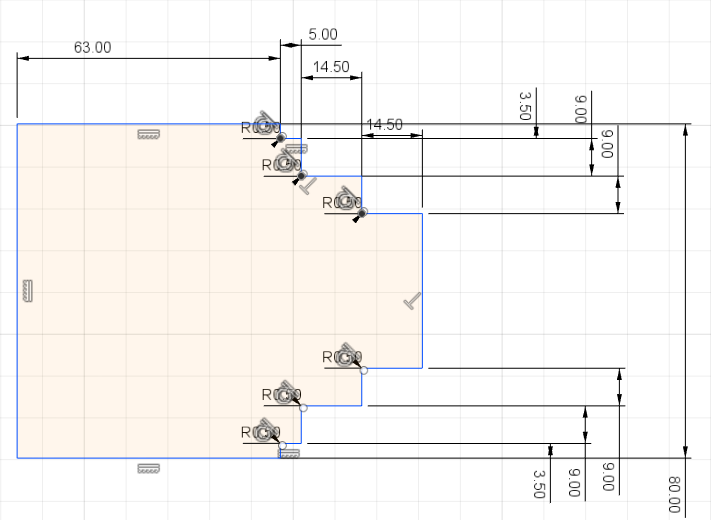
\includegraphics[width=110mm,keepaspectratio]{Figures/Placa1v6.png}
	\caption{Medidas de la placa electrónica.}
	\label{fig:medidaspcb}
\end{figure}

Una vez que fueron establecidas las medidas y el microcontrolador que debía ser usado (un msp430), se delimitó la placa en los dos sectores previamente mencionados. Esta división puede observarse en la figura \ref{fig:pcbbase}, ambas divisiones deberían encontrarse aisladas, por lo que se debía dejar cierto espacio entre el cobre.

\begin{figure}[h]
	\centering
	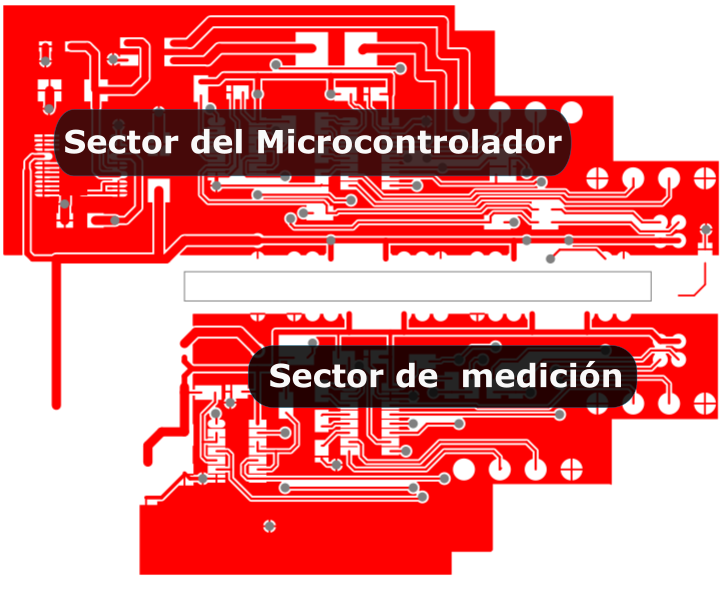
\includegraphics[width=80mm,keepaspectratio]{Figures/esquema22.png}
	\caption{Placa de ejemplo para la aislación.}
	\label{fig:pcbbase}
\end{figure}



La figura \ref{fig:pcbbase} es una vista de un diseño que proveyó la empresa como punto de partida para el desarrollo de los circuitos impresos.

Se estableció entonces que en el sector del microcontrolador se encontrarán los puertos de comunicación y en el sector de medición, los integrados y circuitos analógicos que adapten las entradas a medir.

\subsection{Componentes esenciales}

Basándose en los requerimientos se fue definiendo al dispositivo como  un conjunto de circuitos, estos son:

\begin{itemize}
\item Un circuito de alimentación.
\item Circuito de adaptación de microcontrolador.
\item Circuito de aislación, o de cambio de nivel.
\item Circuito de medición.
\item Circuito de comunicación por puerto.
\item Circuito de relé.
\item Circuito de salida analógica.
\end{itemize}

Todos estos circuitos se encuentran en el sector de microcontrolador que puede verse de la figura \ref{fig:pcbbase}, a excepción del circuito de  medición que se encuentra en el sector de medición  y el circuito de aislación que funciona de interface y se encuentra en ambos sectores.

\subsubsection{Circuito de alimentación}
Se comenzó a realizar el circuito teniendo por presupuesto que la alimentación se haría con una fuente alterna de 8 V a 30 V.

Para la alimentación se optó por una fuente switching  LM2574 que provee 5 V a un regulador lineal de 3,3 V necesarios para operar el microcontrolador. El circuito descrito puede observarse en la figura \ref{fig:circalim1}.

\begin{figure}[h]
	\centering
	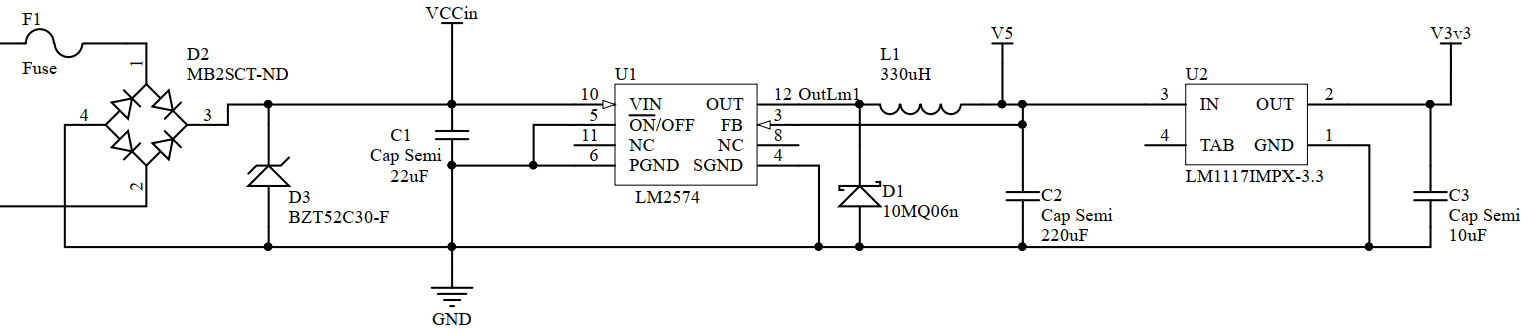
\includegraphics[width=120mm,keepaspectratio]{Figures/alimentacion1.png}
	\caption{Esquemático de la alimentación de la placa.}
	\label{fig:circalim1}
\end{figure}

\subsubsection{Circuito de aislación o de cambio de nivel}
Para proteger al microcontrolador de elevadas tensiones se utilizó un integrado de aislación, un conversor de continua a continua para alimentar el circuito de medición. También se añadió un aislador digital para comunicar el microcontrolador principal con un integrado de medición.

\begin{figure}[h]
	\centering
	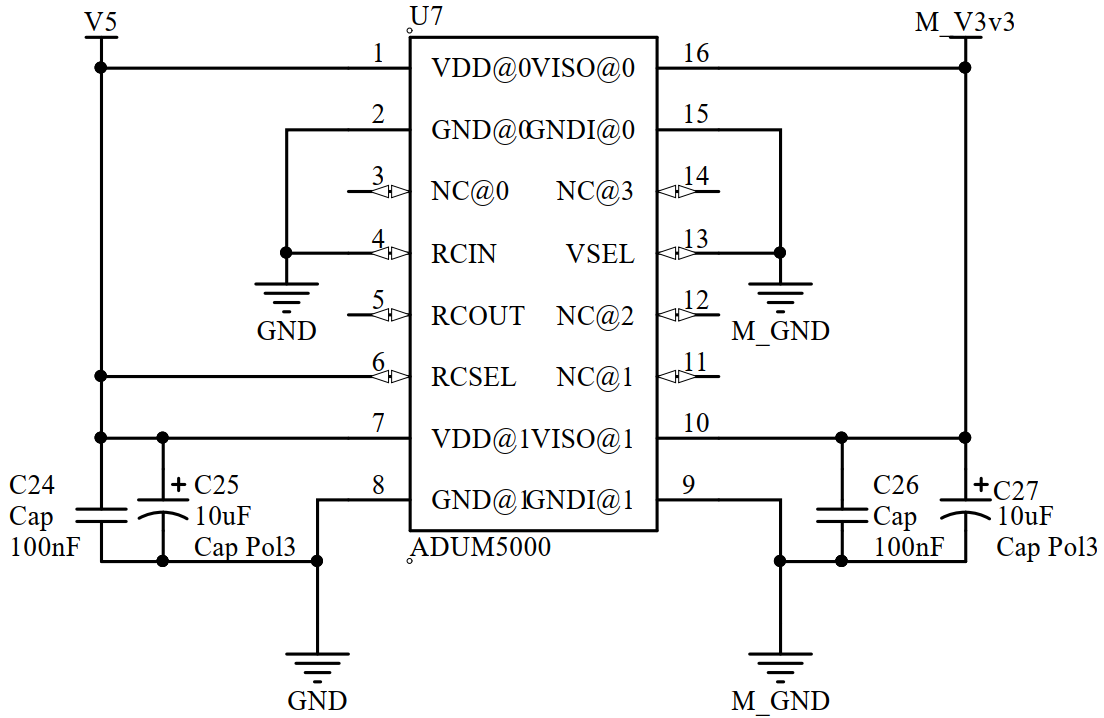
\includegraphics[width=100mm,keepaspectratio]{Figures/alimentacion2.png}
	\caption{Esquemático de la alimentación del sector aislado.}
	\label{fig:circaisl1}
\end{figure}

\begin{figure}[h]
	\centering
	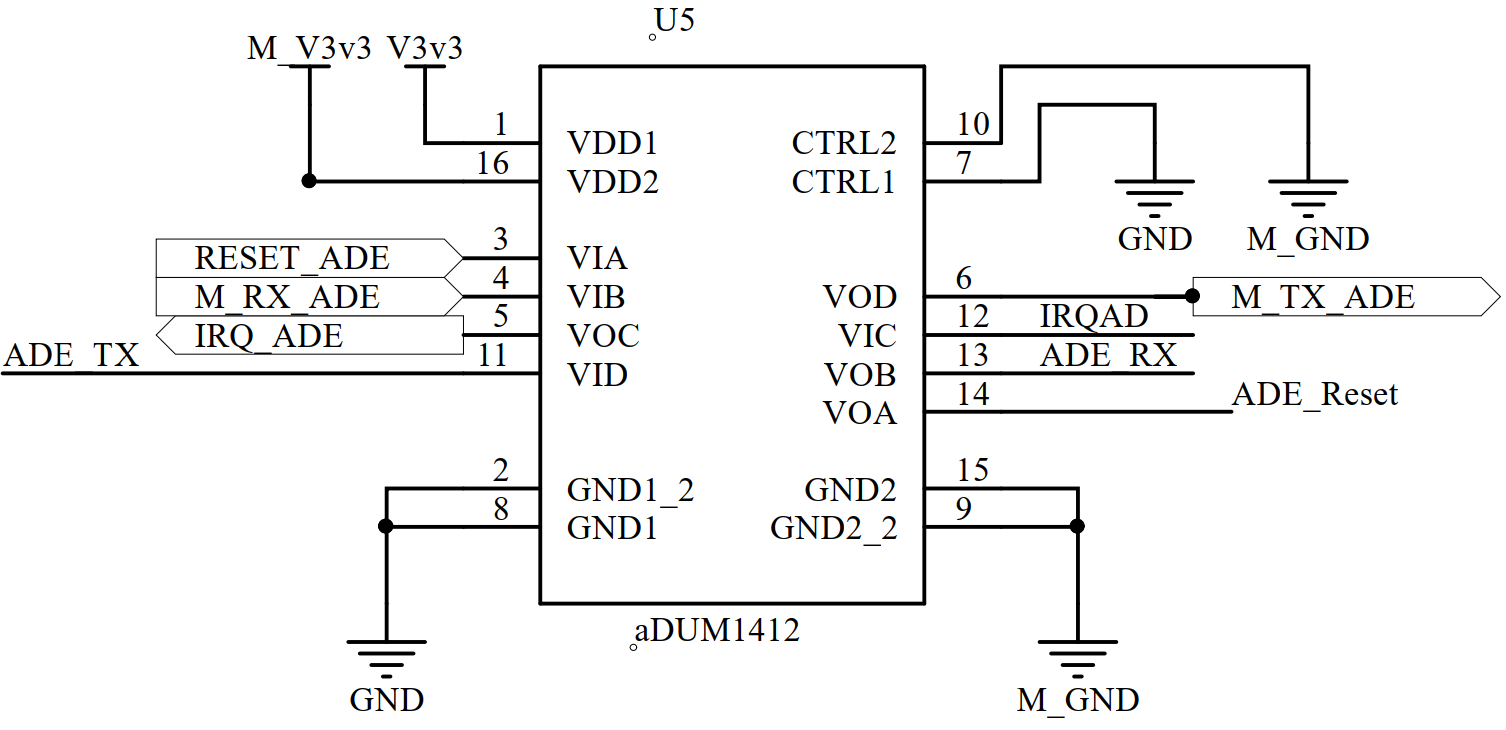
\includegraphics[width=100mm,keepaspectratio]{Figures/comaislado1.png}
	\caption{Esquemático de la comunicacion digital aislada.}
	\label{fig:circaisl2}
\end{figure}

 
\subsubsection{Circuito de adaptación de microcontrolador}

El circuito de adaptación esta integrado por resistores y capacitores necesarios para el correcto funcionamiento del microcontrolador, como tambien un cristal externo para usarlo como oscilador. Se usó un microcontrolador de la familia MSP430, este micro es de uso común en la empresa. 

En el circuito de adaptación se incluyó un semiconductor para tensión de referencia y un cristal de 32768 Hz. Para el armado del dispositivo se seleccionó el modelo msp430F2618, que posee un DAC interno de 12 bit que es de utilidad para la salida analógica utilizada en el lazo de corriente.

Para programar al microcontrolador se añadió una conexión JTAG para conectar un programador flash de la empresa Texas Instrument. Este puerto de salida puede verse en la figura \ref{fig:jitag}.

\begin{figure}[h]
	\centering
	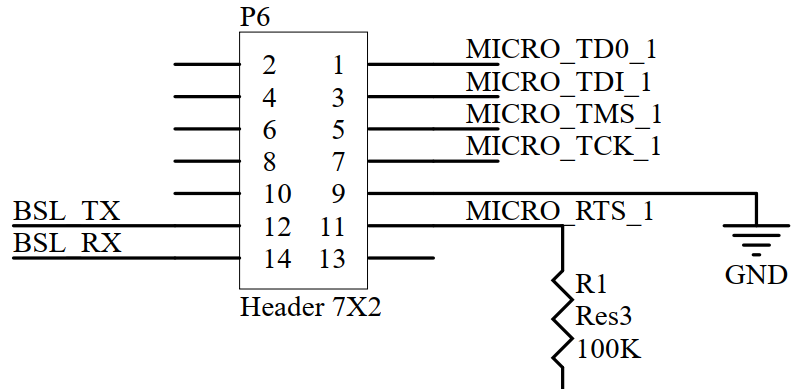
\includegraphics[width=120mm,keepaspectratio]{Figures/JTAG1.png}
	\caption{Header JTAG añadido al PCB.}
	\label{fig:jitag}
\end{figure}

\subsubsection{Circuito de comunicación por puerto}
Como se estableció en los requisitos, se implementaron integrados para la comunicación RS232, un max3222 y para la RS485, un integrado ISL83485. Estos integrados facilitan la adaptación de tensiones para lograr el estándar de comunicación deseado.

\begin{figure}[h]
	\centering
	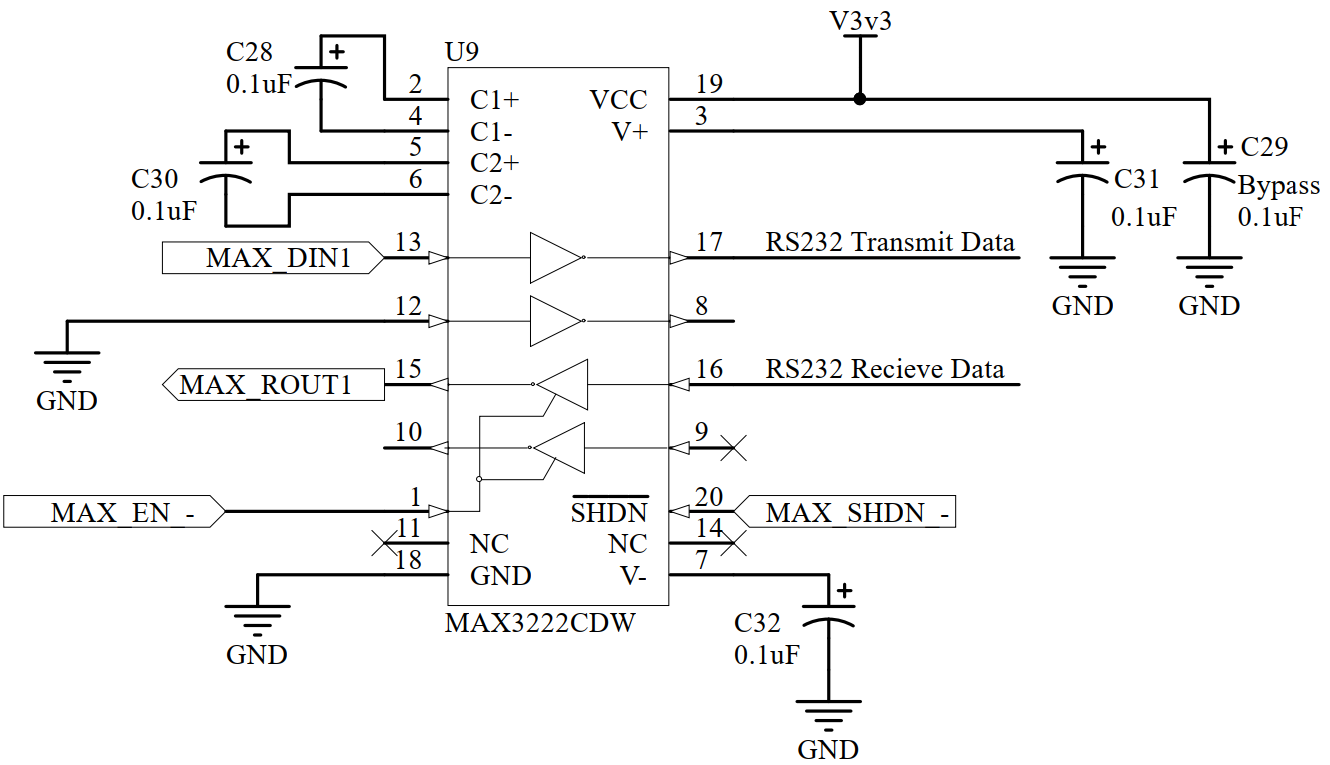
\includegraphics[width=120mm,keepaspectratio]{Figures/RSS232_1.png}
	\caption{Implementación del MAX3222 en el esquemático elaborado.}
	\label{fig:2321esquem}
\end{figure}

\begin{figure}[h]
	\centering
	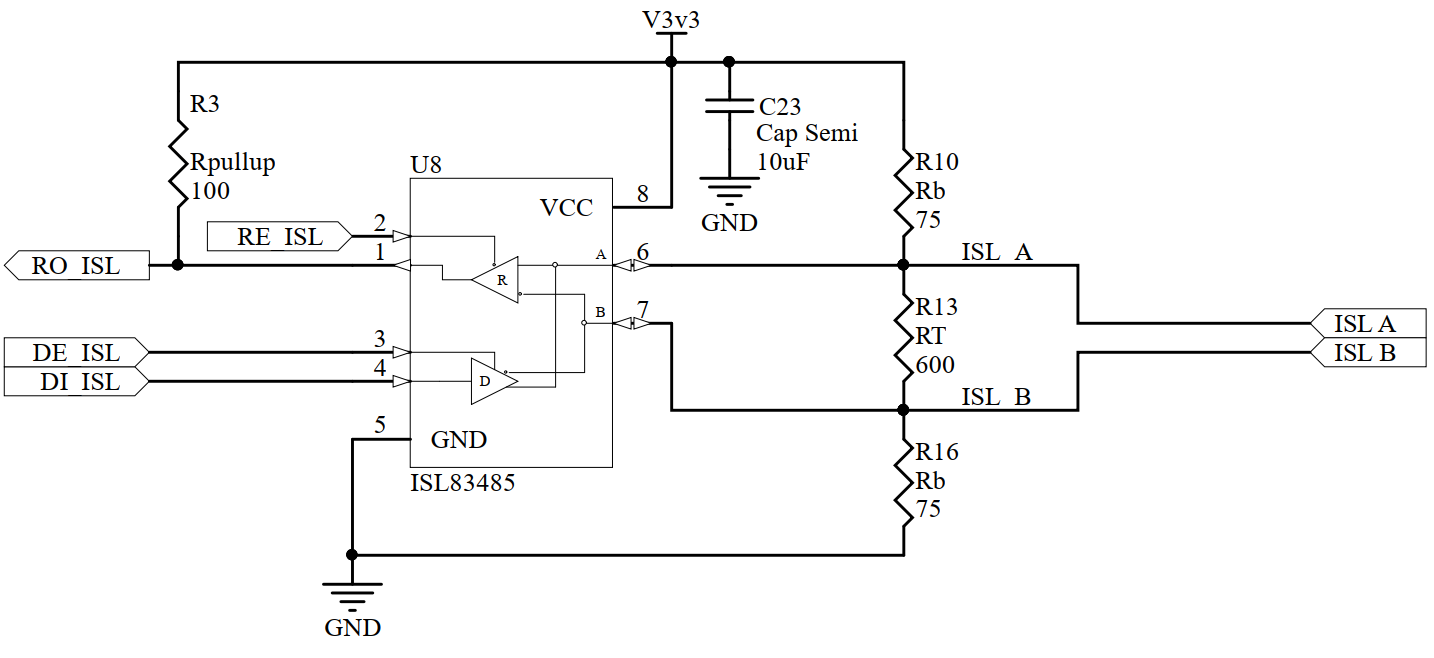
\includegraphics[width=120mm,keepaspectratio]{Figures/RSS485_1.png}
	\caption{Implementación del ISL83485 en el esquemático elaborado.}
	\label{fig:4851esquem}
\end{figure}


\subsubsection{Circuito de relé}
El circuito es integrado por los componentes mínimos para que el microcontrolador pueda manejar un relé que se acciona con tensiones del orden de los 5 volts. El circuito puede verse en la figura \ref{fig:rele1equem}.

\begin{figure}[h]
	\centering
	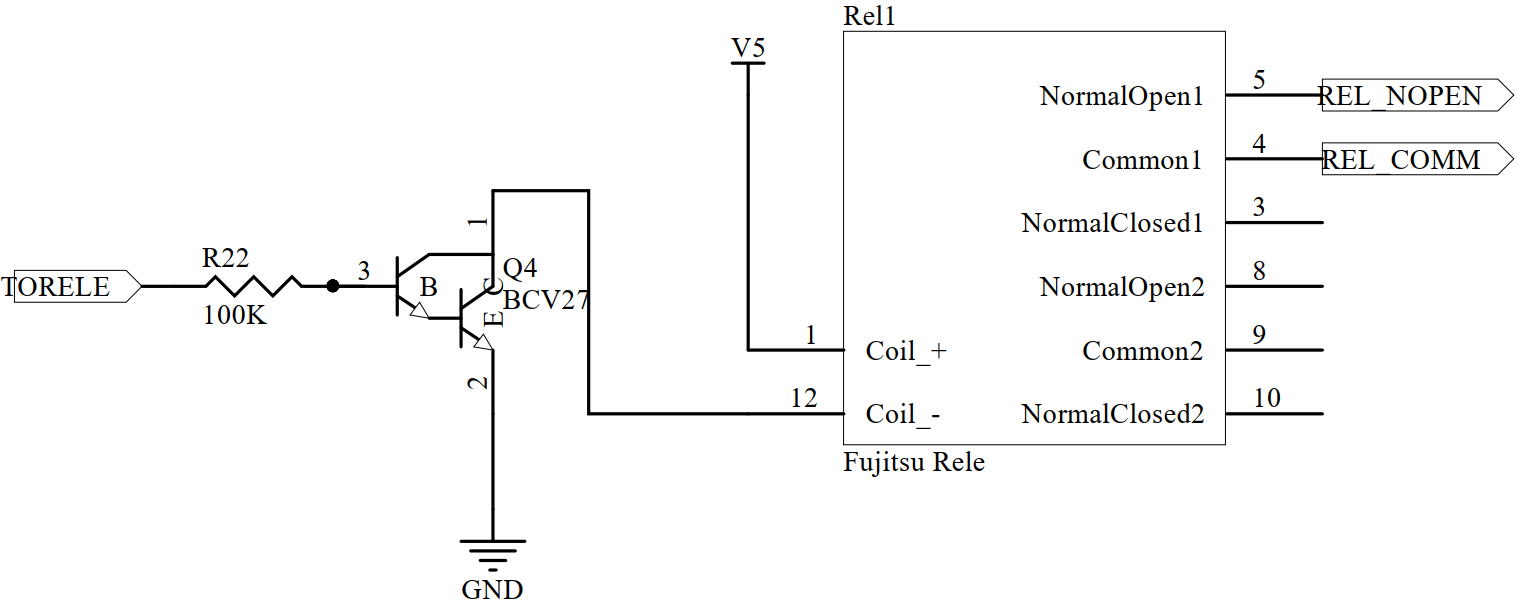
\includegraphics[width=120mm,keepaspectratio]{Figures/rele1.png}
	\caption{Transistor darlington para la acción del relé.}
	\label{fig:rele1equem}
\end{figure}

\subsubsection{Circuito de salida analógica}
Este circuito esta compuesto por un \textit{buffer} combinado con un integrado regulador de corriente para lograr una salida de lazo de corriente 4 - 20 mA.

\begin{figure}[h]
	\centering
	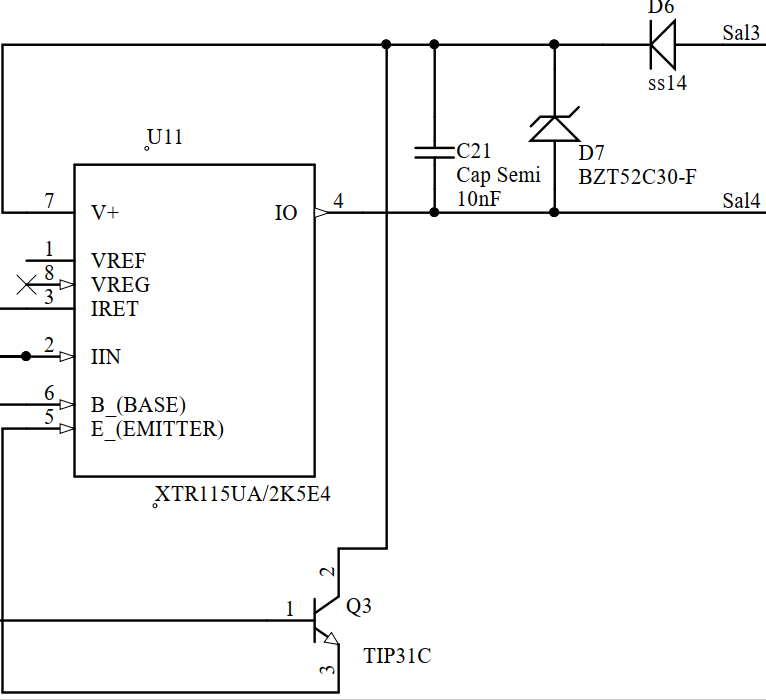
\includegraphics[width=120mm,keepaspectratio]{Figures/salida420.png}
	\caption{Circuito de salida 4 - 20 mA.}
	\label{fig:rele1equem}
\end{figure}


\subsubsection{Circuito de medición}

Para realizar la medición se optó por un integrado miltifuncional de medición de una sola fase. El  integrado permitió la rápida implementación de un medidor en el circuito del dispositivo. El integrado elegido es el ADE7953 del fabricante Texas Instrument. El integrado es un SOC (\textit{system on chip}) que adapta un AFE (\textit{analog front-end} ) para su fácil uso. El esquemático del ADE7953 puede verse en la  figura \ref{fig:ade79esquem}.

\begin{figure}[htb]
	\centering
	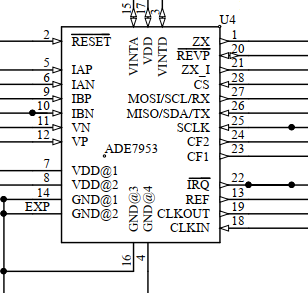
\includegraphics[width=100mm,keepaspectratio]{Figures/ade7953.png}
	\caption{Diagrama de bloque del ADE7953.}
	\label{fig:ade79esquem}
\end{figure}

El integrado de medición puede comunicarse con el microcontrolador por tres diferentes protocolos: I2C, SPI y UART, para esto deben realizarse las conexiones necesarias. Debido a la decisión de aislar el integrado y que las condiciones de espacio no permitían sobrepasarse con la cantidad de integrados para aislar, se realizaron las conexiones para la comunicación UART solamente.

\subsection{Esquema analógico de medición }
Como el principal objetivo del dispositivo es medir, se explica de manera muy breve, los arreglos analógicos que se implementaron.

Suponiendo que las tensiones a medir fuesen del orden de los 600 V y teniendo en cuenta que la máxima tension que soporta un pin del integrado es de 2 V, se añadió una serie de resistores para lograr 1 mega $\Omega$  de resistencia en la entrada de medición, de modo de atenuar la tension. Una vez atenuada la tensión se agrega un divisor resistivo del cual el integrado mide.

\begin{figure}[htb]
	\centering
	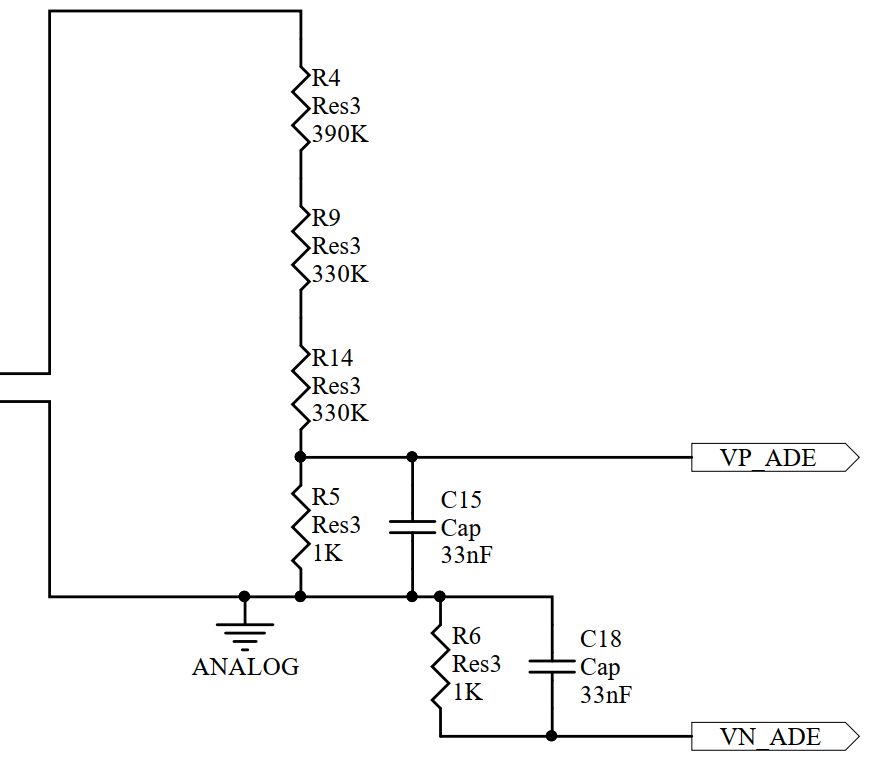
\includegraphics[width=80mm,keepaspectratio]{Figures/medicionvoltaje.png}
	\caption{Esquemático de la entrada de tension.}
	\label{fig:medvolt}
\end{figure}

Para la medición de corriente es común ver en los módulos comerciales el uso de una bobina de Rogowski, sin embargo para el modulo diseñado se optó por usar un \textit{shunt} para que el dispositivo no dependa de otro objeto discreto para su instalación. El \textit{shunt} elegido soporta grandes corrientes y se tomaron precauciones en las pistas del PCB para que pueda operar con normalidad.

\begin{figure}[htb]
	\centering
	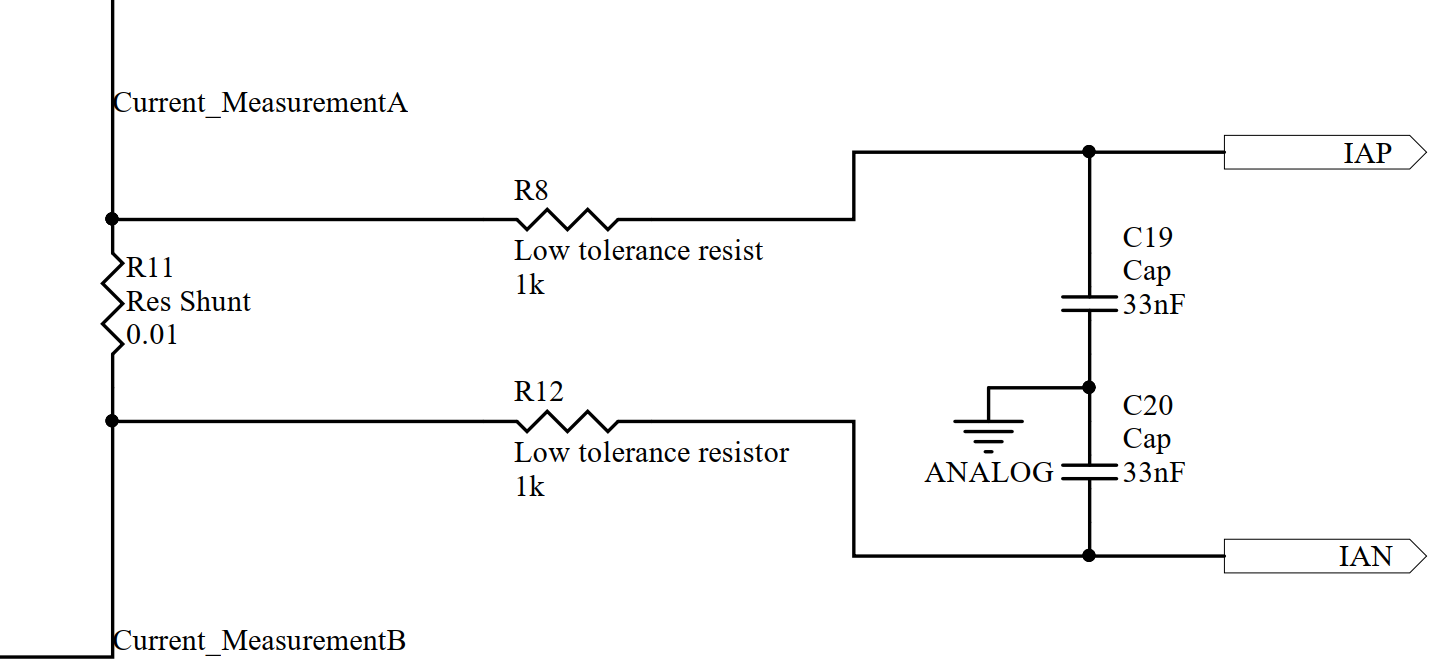
\includegraphics[width=120mm,keepaspectratio]{Figures/medicioncorriente.png}
	\caption{Esquemático de la entrada de corriente.}
	\label{fig:medcurrent}
\end{figure}

\subsection{Fabricación}

Una vez completada la totalidad de las conexiones lógicas en el esquemático, se debía decidir sobre el posicionamiento de los componentes, el tamaño de las perforaciones y la distribución de cada circuito. Se estableció desde la empresa privada que todos los componentes pasivos en lo posible sean de montaje superficial, por lo que la mayoría de resistores y capacitores serian de encapsulado 0805. Un 0805 puede verse en la figura \ref{fig:smd0805}.

\begin{figure}[!h]
	\centering
	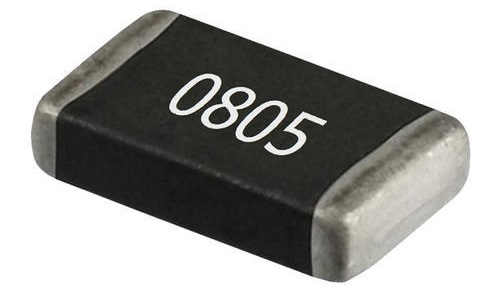
\includegraphics[width=50mm,keepaspectratio]{Figures/smd0805.jpg}
	\caption{Componente de soldadura superficial.}
	\label{fig:smd0805}
\end{figure}

Se dejó espacio para una entrada de conector RJ45 para un futuro puerto LAN ethernet y se delimitó una zona de exclusión para dividir al PCB en una zona de medición y una zona de microcontrolador.

Debido a que el PCB iba a ser encapsulado por una carcasa de plástico con posibilidad de conexión de 16 salidas, se decidió previamente como debería ser el esquema de conexiones. Se dejo un conector de 4 salidas para las mediciones ya que este se encontraría en un nivel aislado.

\begin{figure}[h]
	\centering
	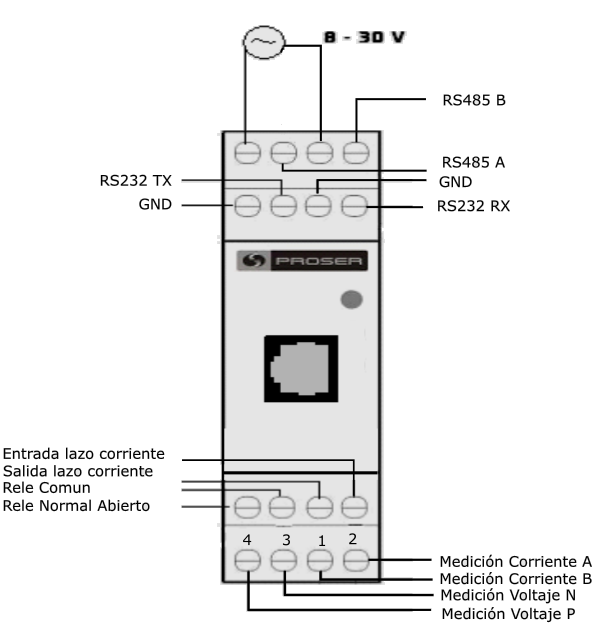
\includegraphics[width=120mm,keepaspectratio]{Figures/conectores2.png}
	\caption{Salidas del dispositivo.}
	\label{fig:salidas01}
\end{figure}

Se decidió fabricar las placas electrónicas en Argentina. La empresa fabricante tiene publicada una tabla donde divulga con qué tipos de tecnología de fabricación trabaja. Se estableció como estándar a usar el de 8 milis y se trabajó con ese limite en el CAD de diseño.

\begin{figure}[htb]
	\centering
	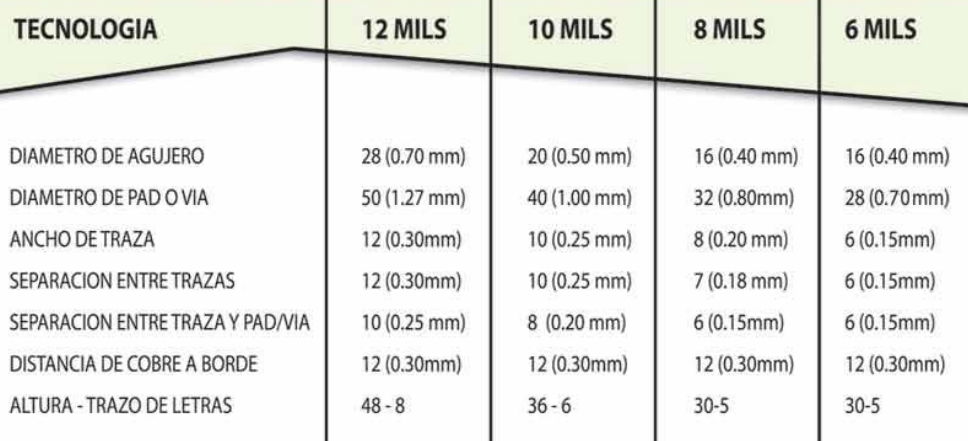
\includegraphics[width=110mm,keepaspectratio]{Figures/estandaresmayer.png}
	\caption{Estandares fijados por la empresa argentina Ernesto Mayer SA.}
	\label{fig:mayerstandar}
\end{figure}

El resultado del diseño puede verse en la figura \ref{fig:PCBfrontt}, que es la cara superior de la placa donde se encuentran la mayoría de los componentes. 

\begin{figure}[h]
	\centering
	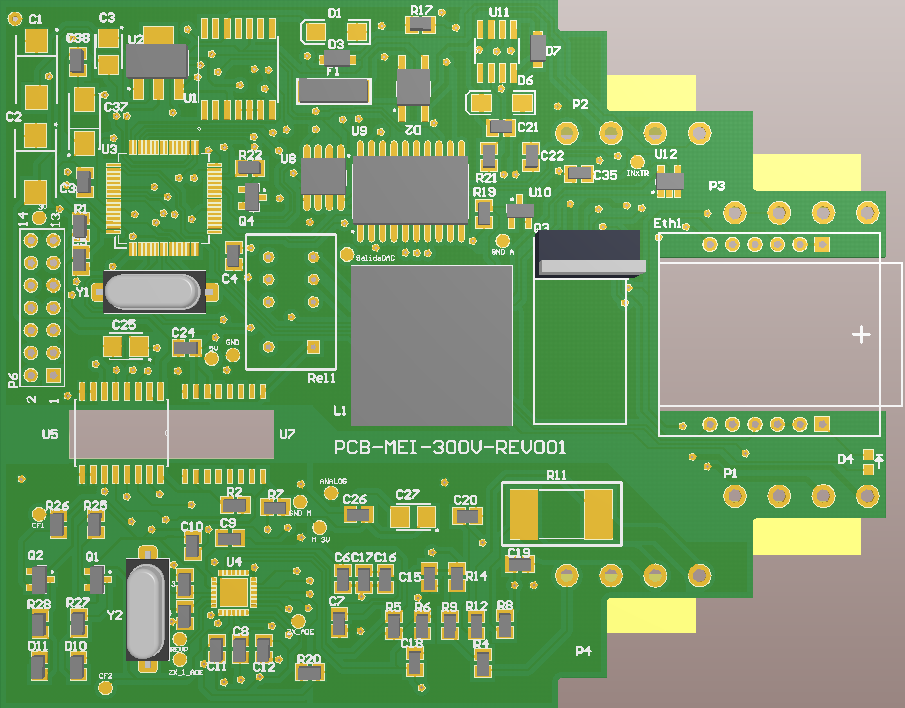
\includegraphics[width=110mm,keepaspectratio]{Figures/PCBfront.png}
	\caption{Imagen 3D de la parte frontal del PCB.}
	\label{fig:PCBfrontt}
\end{figure}

La cara inferior puede verse en la figura \ref{fig:PCBbackk}. Como esta cara se soldaría por refusión de una ola de estaño que viene de izquierda a derecha, tal como se ve a la imagen, se minimizó la cantidad de integrados en ella y se acomodaron los \textit{footprints} para que no queden puntos ciegos sin soldar.

\begin{figure}[htb]
	\centering
	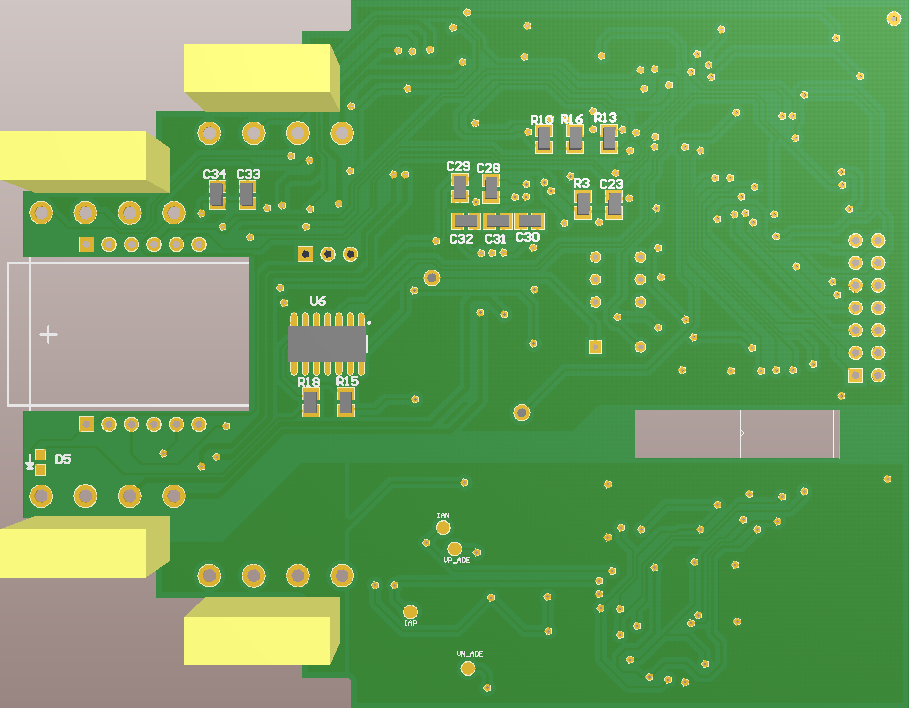
\includegraphics[width=110mm,keepaspectratio]{Figures/PCBback.png}
	\caption{Imagen 3D de la parte trasera del PCB.}
	\label{fig:PCBbackk}
\end{figure}


\section{Desarrollo de \textit{software}}
Se desarrollo un software para e uso del dispositivo armado, es decir se desarrollo un programa en c para descargarlo al microcontrolador y que este realice todas las tareas necesarias.

\subsection{Software previos de base}
Se desarrollo durante la cursada de la especialización un programa en lenguaje c para implementarlo en un microntrolador LPC4337 para hacer uso de un circuito integrado wiznet w5500, que es un controllador ethernet que maneja protocolo TCP/IP, comunmente utilizado para realizar una conecxion a internet de manera sencilla. Se penso en el desarrollo de este programa para implementarlo al futuro puerto ethernet del dispositivo.

También se habían desarrollado como parte de las materias de la especialización programas simples de bucle infinito con interrupción para la introducción de sistemas operativos, uno de estos programas fue usado como base para la elaboración del programa final.


\subsection{Microcontrolador Principal}
El microcontrolador elegido para el dispositivo fue un MSP430F2618 fabricado por la empresa Texas Instrument, este microcontrolador es de ultra baja potencia con una CPU de instrucciones RISC de 16 bits. Posee periféricos analógicos y digitales orientado a aplicaciones de medición. Este microcontrolador puede pasar de varios modos de baja potencia a modo activo en menos de 1 microsegundo.

\begin{figure}[!h]
	\centering
	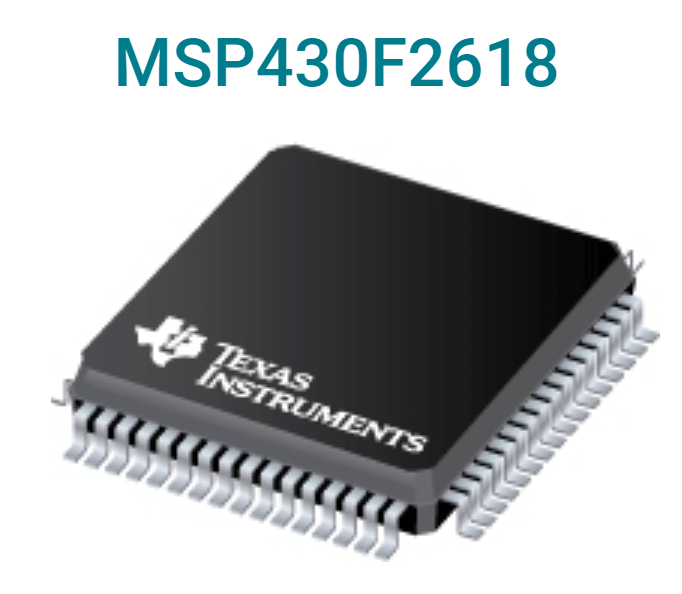
\includegraphics[width=40mm,keepaspectratio]{Figures/msp430F2618.png}
	\caption{Ilustración del micro controlador como se lo presenta en la pagina web del fabricante.}
	\label{fig:msp430imagen}
\end{figure}

Para realizar el programa en lenguaje c y descargarlo en el microcontrolador la empresa SERVAIND S.A. proveyó un entorno de desarrollo privado y una placa electrónica con el microcontrolador funcionando, de modo de probarla. Una ventana del entorno de desarrollo puede verse en la figura \ref{fig:IARwindow}.

\begin{figure}[h]
	\centering
	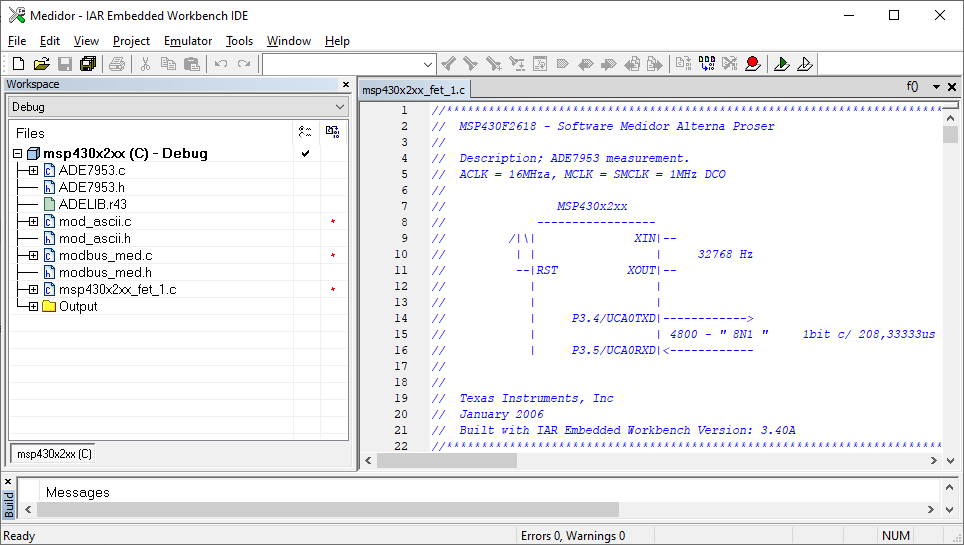
\includegraphics[width=110mm,keepaspectratio]{Figures/Embeddedworkbench.png}
	\caption{Imagen del entorno de desarrollo.}
	\label{fig:IARwindow}
\end{figure}



\subsection{Especificaciones del software desarrollado}

Ante la necesidad de realizar un software robusto y de uso instrumental se deseaba implementar un FreeRTOS pero  debido a limitaciones de memoria del microcontrolador resultaba inviable implementarlo, por lo que se decidió realizar un programa \textit{bare metal}.

El software realizado consiste en un bucle infinito controlado por tiempo(1 milisegundo) usando uno de los dos timers internos del microcontrolador. La principal tarea del programa es comunicarse constantemente con el integrado de medición \textbf{ADE7953} y almacenar los datos de sus registros en la memoria local. Dentro del periodo de un milisegundo que dura el barrido del bucle se realizan otras tareas como comunicar datos a otros puertos, accionar el relé o cambiar los leds.

\subsubsection{Comunicacion con el ADE7953}

La comunicación con el ADE7953 se realiza por UART por medio de un protocolo establecido por el fabricante del chip. Como la comunicación UART del chip esta fijada en 4800 bps cada frame que se le envía tiene un tiempo de 2.08 ms, el tiempo entre cada frame es de 0.2 ms a 4ms (t1) como máximo y el tiempo de espera entre cada comunicación exitosa es de 6ms (t2).

El ADE7953 tiene registros internos de 8, 16 y 24 bits donde almacena información de medición y de configuración para su funcionamiento, estos registros son tanto de escritura como de lectura. La dirección  de registros de 8 bits puede verse en la tabla \ref{8biadcregis}.

Las operaciones de lectura con el ADE7953 puede verse en la figura \ref{fig:ADEread}, para leer un registro debe primeramente enviarse un byte de valor 0x35 y luego los bytes de la dirección del registro a leer, para luego recibir la cantidad de bytes según el tamaño del registro solicitado.

\begin{figure}[htb]
	\centering
	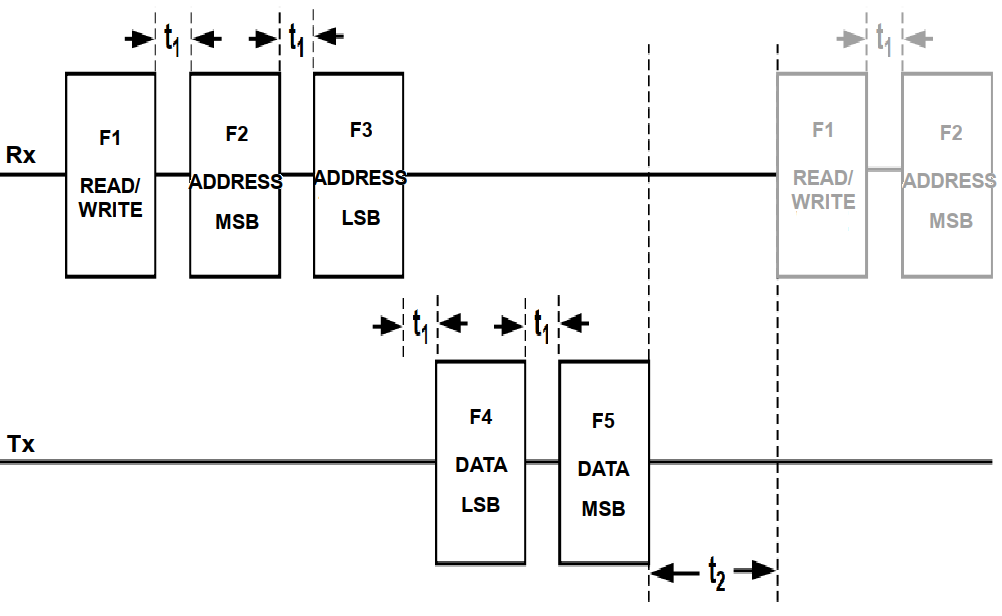
\includegraphics[width=110mm,keepaspectratio]{Figures/ade7uartread.png}
	\caption{Lectura por UART del ADE7953.}
	\label{fig:ADEread}
\end{figure}

Para la operación de escritura del ADE7953 debía enviarse un byte con el valor 0xCA ,luego los bytes de la dirección a escribir y por ultimo los datos en la misma cantidad de \textit{frames} que espacio del registro, como puede observarse en la figura \ref{fig:ADEwrite}.

\begin{figure}[htb]
	\centering
	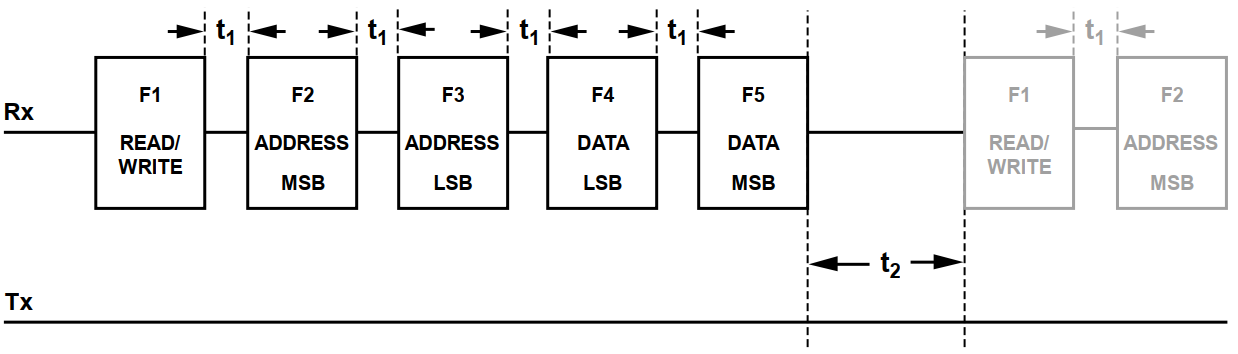
\includegraphics[width=110mm,keepaspectratio]{Figures/ade7uartwrite.png}
	\caption{Escritura por UART del ADE7953.}
	\label{fig:ADEwrite}
\end{figure}

Se configuro al programa de tal modo que lea los registros necesarios para monitorear la potencia eléctrica de la maquina donde se lo instale, los registros que el programa lee y almacena son:

\begin{itemize}
\item AVA\_ 24 Potencia aparente instantánea. 
\item AWATT\_ 24 Potencia activa instantánea.
\item AVAR\_ 24 Potencia reactiva instantánea. 
\item IA\_ 24 Corriente instantánea.
\item V\_ 24 Voltaje instantáneo.
\item IRMSA\_ 24 Corriente RMS.
\item VRMS\_ 24 Voltaje RMS.
\item AENERGYA\_ 24 Energia activa.
\item RENERGYA\_ 24 Energia reactiva.
\item APENERGYA\_ 24  " Energía Aparente".
\item VPEAK\_ 24 Pico de voltaje.
\item PFA\_ 16 Factor de potencia.
\item Period\_ 16 Registro de período.
\end{itemize}


El programa tarda aproximadamente un total de 241 ms en leer la totalidad de estos registros usando el protocolo elegido, por lo que queda un amplio margen para realizar otras operaciones.


\begin{table}[h]
\centering
\caption[Registros 8 bit ADE79853]{Registros de 8 bit del ADE7953 como se los muestran en el \textit{datasheet} del fabricante.}
\begin{tabular}{@{}llllll@{}}
\hline
Address & Register Name  & R/W & Default & Type     & Register Description                                                                                                                                 \\ \hline
0x000   & SAGCYC         & R/W & 0x00    & Unsigned & Sag line cycles                                                                                                                                      \\
0x001   & DISNOLOAD      & R/W & 0x00    & Unsigned & No-load detection disable                                                                                                                            \\
0x004   & LCYCMODE       & R/W & 0x40    & Unsigned & \begin{tabular}[c]{@{}l@{}}Line cycle accumulation mode \\ configuration\end{tabular}                                                                \\
0x007   & PGA\_V         & R/W & 0x00    & Unsigned & \begin{tabular}[c]{@{}l@{}}Voltage channel \\ gain configuration (Bits{[}2:0{]})\end{tabular}                                                        \\
0x008   & PGA\_IA        & R/W & 0x00    & Unsigned & \begin{tabular}[c]{@{}l@{}}Current Channel A\\  gain configuration (Bits{[}2:0{]})\end{tabular}                                                      \\
0x009   & PGA\_IB        & R/W & 0x00    & Unsigned & \begin{tabular}[c]{@{}l@{}}Current Channel B gain \\ configuration (Bits{[}2:0{]})\end{tabular}                                                      \\
0x040   & WRITE\_PROTECT & R/W & 0x00    & Unsigned & \begin{tabular}[c]{@{}l@{}}Write protection bits\\  (Bits{[}2:0{]})\end{tabular}                                                                     \\
0x0FD   & LAST\_OP       & R   & 0x00    & Unsigned & \begin{tabular}[c]{@{}l@{}}Contains the type \\ (read or write) \\ of the last successful \\ communication\\ (0x35 =read; 0xCA = write)\end{tabular} \\
0x0FF   & LAST\_RWDATA   & R   & 0x00    & Unsigned & \begin{tabular}[c]{@{}l@{}}Contains the data from \\ the last successful 8-bit\\  register communication\end{tabular}                                \\
0x702   & Version        & R   & N/A     & Unsigned & \begin{tabular}[c]{@{}l@{}}Contains the silicon\\  version number\end{tabular}                                                                       \\
0x800   & EX\_REF        & R/W & 0x00    & Unsigned & \begin{tabular}[c]{@{}l@{}}Reference input \\ configuration: set\\  to 0 for internal; \\ set to 1 for external\end{tabular}                         \\ \hline
\end{tabular}
\label{8biadcregis}
\end{table}




\subsection{Funcionalidades del software}
El software maneja un menú por el cual una terminal puede comunicarse con el programa por medio de un puerto serie para realizar determinadas configuraciones.

Al iniciar el programa, dentro de los primeros 10 segundos se puede enviar unos caracteres en código ANSII (las letras cfg) y el programa inicia un menú, enviando caracteres con las opciones. Este menú puede verse en la figura  \ref{fig:menumanual}.

El menú puede mostrar las variables que se están midiendo configurar el puerto serie, modificar a que variable depende la salda del bucle analógico y activar una alarma que acciona al relé dependiendo de una variable seleccionada.

\begin{figure}[!htb]
	\centering
	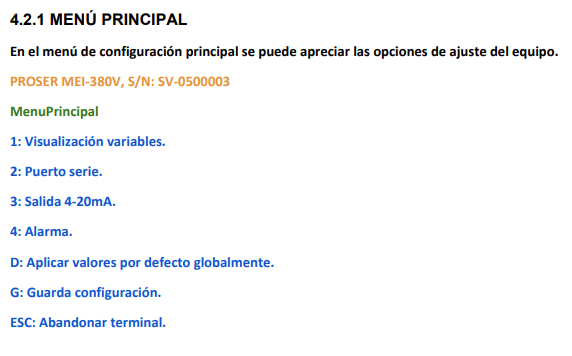
\includegraphics[width=110mm,keepaspectratio]{Figures/menumanual.png}
	\caption{Menú serie en el manual.}
	\label{fig:menumanual}
\end{figure}

\begin{figure}[!htb]
	\centering
	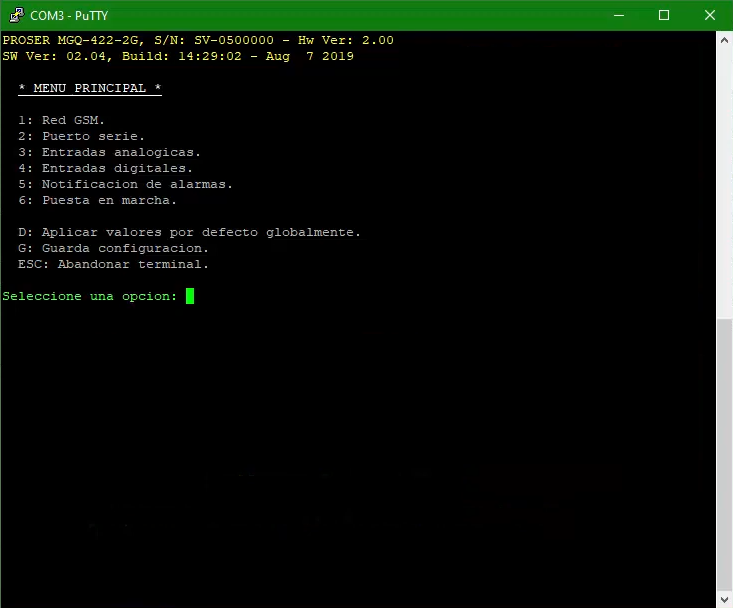
\includegraphics[width=110mm,keepaspectratio]{Figures/menudispositivo07.png}
	\caption{Menú serie ejemplo.}
	\label{fig:serialmenu}
\end{figure}

El software almacena en la memoria del programa valores de medición para poder comunicarlos ya sea por los puertos serie o el enlace de corriente.

El software que controla la placa maneja protocolo modbus para comunicar registros internos en 2 diferentes puertos de interfaces rs232 y 485 según sean seleccionados. Para implementarlo se siguió como referencia el "Modicon Modbus Protocol Reference Guide PI–MBUS–300" y un \textit{driver} libre, el freemodbus.

El modo de acceder a los datos por modbus es solicitando registros que el software maneja, la direccion de los registros puede verse en la tabla\ref{registrosmodbs}.

\begin{table}[h]
\caption[Registros modbus en software]{Registros generados para la comunicación modbus.}
\begin{tabular}{@{}lllll@{}}
\toprule
\begin{tabular}[c]{@{}l@{}}Dirección \\ del \\ Registro\end{tabular} & \begin{tabular}[c]{@{}l@{}}Número \\ del\\ parámetro\end{tabular} & Descripción                    & Unidades & Tipo de dato \\ \midrule
7001                                                                 & 1                                                                 & Voltaje Instantaneo            & Volts    & Float 32     \\
7003                                                                 & 2                                                                 & Voltaje rms                    & Volts    & Float 32     \\
7005                                                                 & 3                                                                 & Corriente instantánea          & Ampere   & Float 32     \\
7007                                                                 & 4                                                                 & Corriente rms                  & Ampere   & Float 32     \\
7009                                                                 & 5                                                                 & Potencia activa                & Watt     & Float 32     \\
7011                                                                 & 6                                                                 & Potencia reactiva              & VA       & Float 32     \\
7013                                                                 & 7                                                                 & Factor de potencia             & -        & Float 32     \\
7015                                                                 & 8                                                                 & Frecuencia                     & Hz       & Float 32     \\
7017                                                                 & 9                                                                 & Energía reactiva medida        & Joules   & Float 32     \\
7019                                                                 & 10                                                                & Energía activa Total acumulada & kWh      & Float 32    
\end{tabular}
\label{registrosmodbs}
\end{table}

EL sofware  maneja una salida para una conexión de lazo de corriente de 4 a 20 mili amperes que es un estándar en la industria para el control de procesos,  el programa puede hacer que esta salida sea proporcional a una variable de medición que puede seleccionarse en el menú serie de configuración.

% Chapter Template

\chapter{Ensayos y resultados} % Main chapter title
\label{Chapter4} % Change X to a consecutive number; for referencing this chapter elsewhere, use \ref{ChapterX}

En este capítulo se explican los diferentes ensayos y tareas que se realizaron para testear tanto el software desarrollado como el hardware fabricado.

%----------------------------------------------------------------------------------------
%	SECTION 1
%----------------------------------------------------------------------------------------

\section{Pruebas Realizadas}
\label{sec:pruebasHW}

Todas las pruebas realizadas se hicieron sobre el prototipo diseñado, que fue fabricado por la empresa Servaind SA. Debido a que la empresa se encuentra radicada en CABA, todas las pruebas con el prototipo fabricado fueron realizadas a distancia por medio de conexiones remotas.

\subsection{Pruebas de comunicación con el ADE7953}
En el inicio del desarrollo del software, se realizaron pruebas midiendo los pines de comunicación entre el microcontrolador y el ADE7953.

Una vez armada la comunicación dentro del programa, se midieron los tiempos de la trama de mensaje UART con un osciloscopio. También se realizaron pruebas de tiempo realizando una serie de pulsos cada milisegundo, la señal puede verse en la figura \ref{fig:Osciloscopp}.


%\begin{figure}[!htb]
%	\centering
%	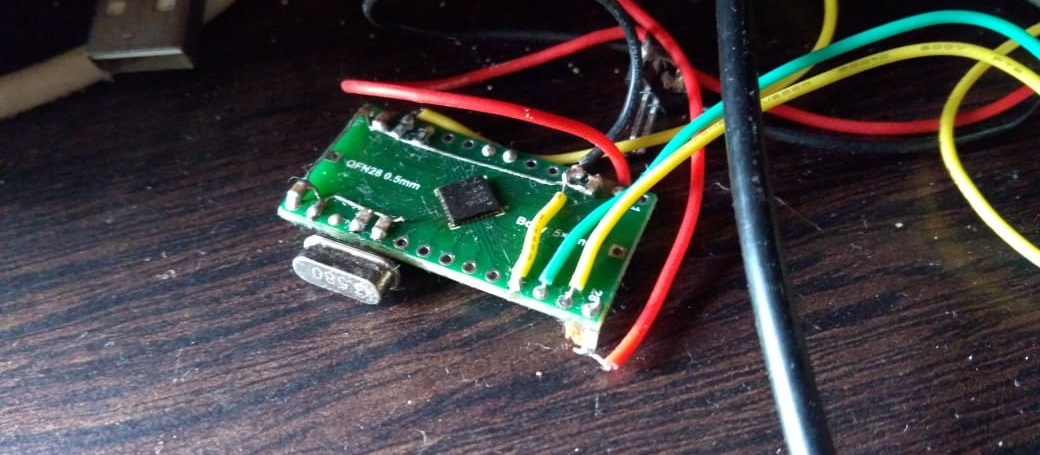
\includegraphics[width=120mm,keepaspectratio]{Figures/ADEadapt.jpg}
%	\caption{ ADE7953 soldado a adaptador.}
%	\label{fig:Adeadapt}
%\end{figure}

\begin{figure}[!htb]
	\centering
	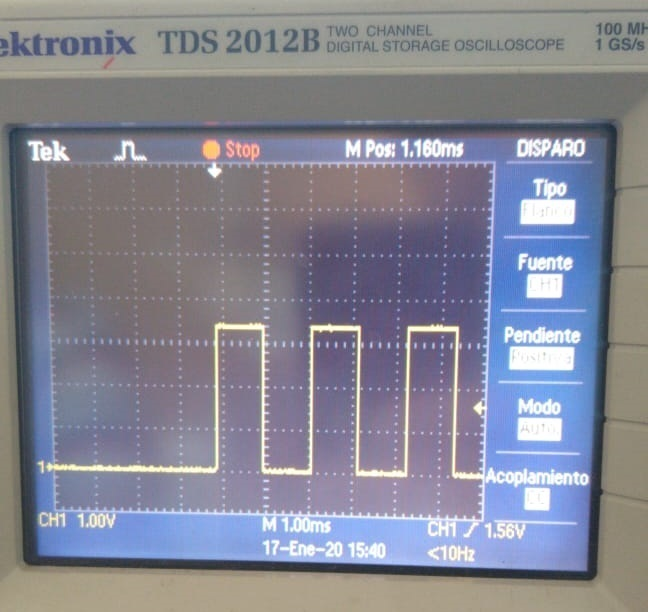
\includegraphics[width=80mm,keepaspectratio]{Figures/osciloscope.jpg}
	\caption{ Pulso de 1 milsegundo en el Osciloscopio.}
	\label{fig:Osciloscopp}
\end{figure}

En el osciloscopio se verificó que los tiempos de la trama fueran los correctos, siguiendo el esquema de la figura \ref{fig:ADEread}. Con el debugger del MSP430 se verificaron las respuestas en los registros. Se enviaron tramas para que el ADE7953 responda los registros de la tabla \ref{8biadcregis}, en la figura \ref{fig:ADEresp} se ve en la memoria del programa la respuesta al registro LAST\_ OP durante las pruebas.



\begin{figure}[!htb]
	\centering
	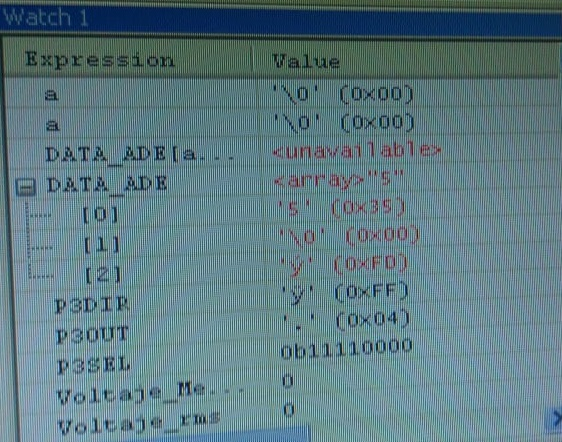
\includegraphics[width=100mm,keepaspectratio]{Figures/ADEresponse.jpg}
	\caption{ Variables leídas por el microcontrolador durante las pruebas.}
	\label{fig:ADEresp}
\end{figure}



\subsection{Testeo del protocolo Modbus}

Una vez finalizado el desarrollo del protocolo Modbus, se procedió a conectar por el puerto RS232 de la placa a la computadora del banco de trabajo. Se leyeron todos los registros disponibles. Esto puede verse en la figura \ref{fig:ModPC}. 

\begin{figure}[!htb]
	\centering
	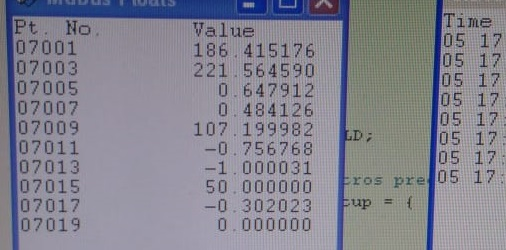
\includegraphics[width=100mm,keepaspectratio]{Figures/ModbusTest.jpg}
	\caption{ Lectura de registros Modbus en la computadora del banco de pruebas.}
	\label{fig:ModPC}
\end{figure}

Se forzaron errores para observar si el software respondía adecuadamente. Los errores probados fueron:

\begin{itemize}
\item Función ilegal
\item Dirección de dato ilegal
\item Valor de dato ilegal
\end{itemize}

Luego se testeo el mismo protocolo sobre la interfaz RS485 para asegurar que no hubiera ninguna diferencia con la interfaz RS232. Gracias a esta segunda prueba se había detectado errores en el software, la biblioteca se inicializaba cada 2 milisegundos. Al finalizar las pruebas, todos  los errores encontrados fueron corregidos.


\subsection{Testeo de la calibración}

Finalizado el desarrollo del  menú principal dentro del programa, se procedió a testear las mediciones que realizaba el dispositivo con un variador de tensión alterna y una carga conocida.
La carga conocida usada fue una lámpara de 100 W. Esta fue utilizada principalmente durante el desarrollo del programa al interpretar los valores de los registros de medición del ADE7953.
 
El variador de tensión alterna puede verse en la figura \ref{fig:BancCalib}. Este fue utilizado al finalizar el desarrollo para realizar pruebas con respecto a la calibración. Se conectó el variador al dispositivo y se probaron diferentes rangos de tensión, realizando pequeños incrementos y verificando con un multímetro. Las mediciones fueron comparadas con un multímetro digital \textquotedblleft Gw Instek Gdm360\textquotedblright.

\begin{figure}[!htb]
	\centering
	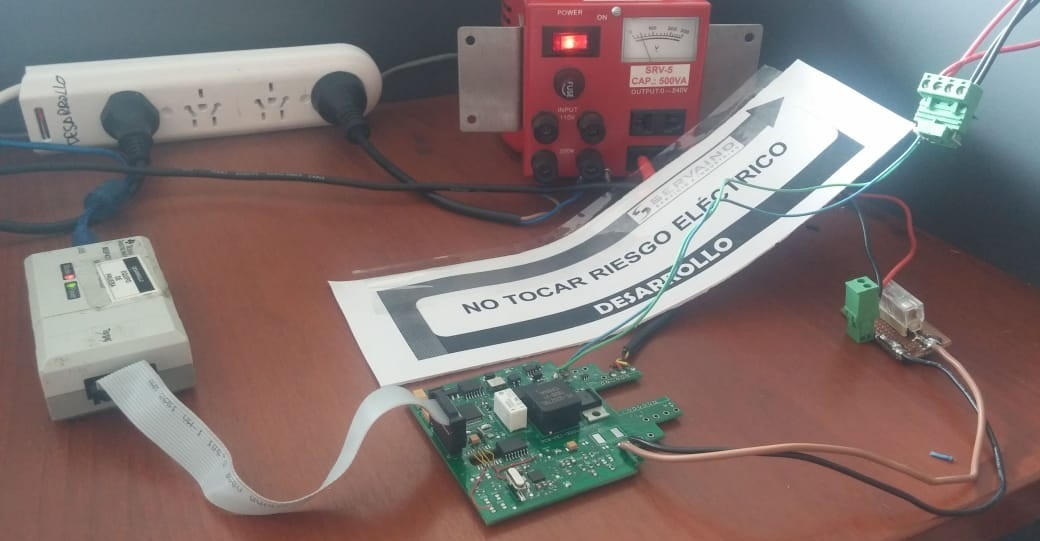
\includegraphics[width=\textwidth ,keepaspectratio]{Figures/BancoCalib.jpg}
	\caption{ Banco de pruebas con el autotransformador.}
	\label{fig:BancCalib}
\end{figure}

Los procedimientos para realizar la calibración fueron los recomendados por la hoja de aplicación del fabricante, se imitó el esquema de la figura \ref{fig:SquemCalib}.

\begin{figure}[!htb]
	\centering
	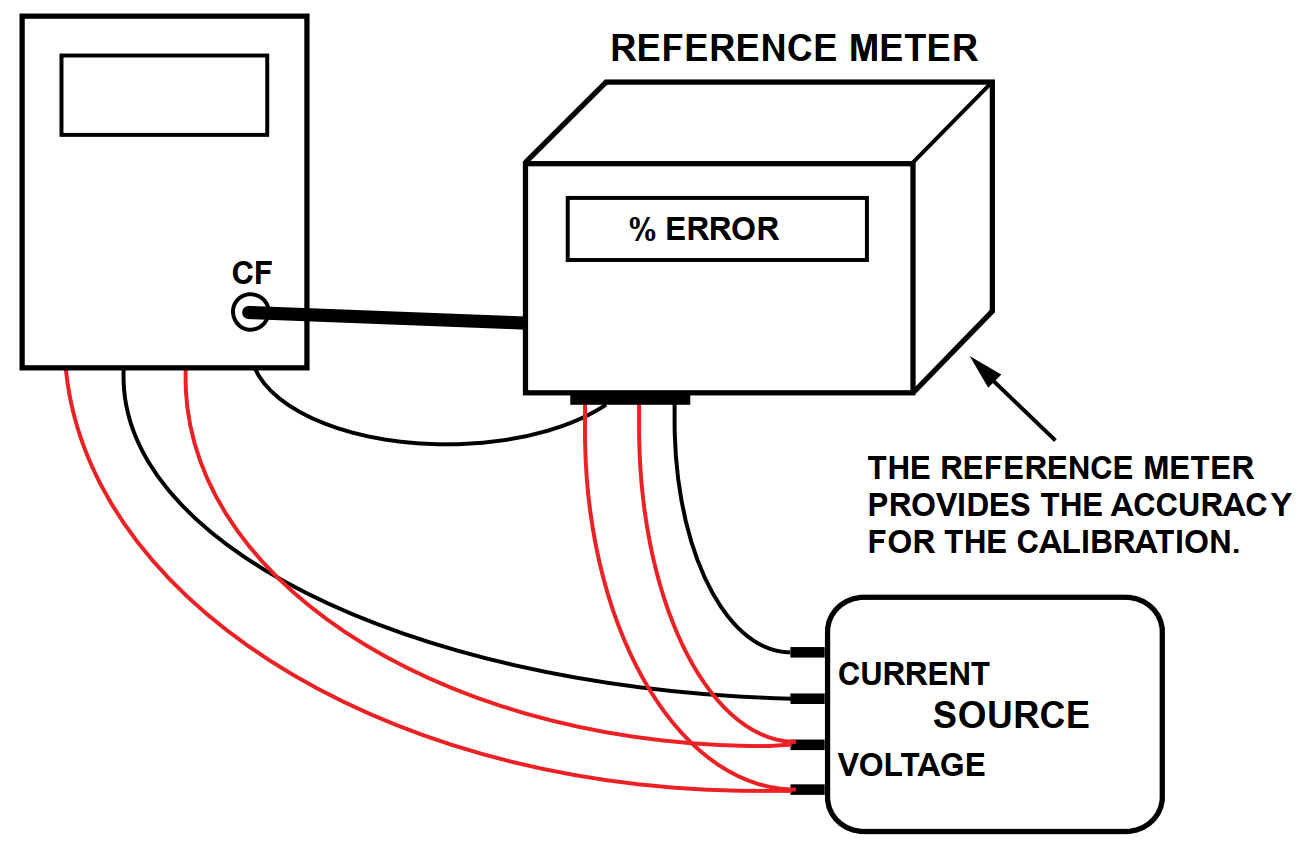
\includegraphics[width=120mm ,keepaspectratio]{Figures/HojadeAplicacion.png}
	\caption{ Esquema de calibración según la hoja de aplicación del integrado ADE7953. La hoja de aplicación denominada AN-1118, se encuentra disponible en la pagina web del fabricante\protect\footnotemark .}
	\label{fig:SquemCalib}
\end{figure}

\footnotetext{\url{https://www.analog.com/media/en/technical-documentation/application-notes/AN-1118.pdf}}

%Se utilizo el primer prototipo para hacer las pruebas. Se realizaron mediciones sobre una lampara de 100 W para probar el funcionamiento del integrado de medición y las funcionalidades del software.

%Se probo desconectar y conectar las tensiones de entrada para probar la reacción de la placa y corregir problemas que presentara en el software. Gracias a esto se detectaron errores en la comunicación 

%Se utilizaron los puertos RS232 y RS485 para probar la comunicación por protocolo modbus.

\section{ Verificación de requerimientos}

%Durante las pruebas se verificaron los requerimientos solicitados.

\subsection{Grupo de requerimientos referidos a alimentación eléctrica}
%\begin{itemize}
%\item El dispositivo deberá alimentarse con tensión continua. La tensión de alimentación deberá ser inferior a 30 V y superior a 12V.
%\end{itemize}

Se conectó el prototipo a un variador de alimentación para probar las diferentes tensiones que soporta para encenderse. Para probar su conector de alimentación, se lo conecto con un fusible. Esto puede verse en la figura \ref{fig:ConectorProoto}.



\begin{figure}[!htb]
	\centering
	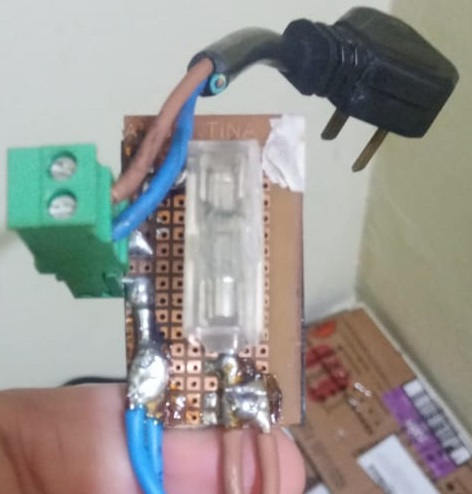
\includegraphics[width=80mm ,keepaspectratio]{Figures/ConectorAlim.jpeg}
	\caption{ Conexión del prototipo durante las pruebas.}
	\label{fig:ConectorProoto}
\end{figure}

\subsection{Grupo de requerimientos referidos a medición de potencia del equipo}

En el prototipo fabricado se implementó una resistencia shunt de 4 mili ohms para realizar mediciones hasta 10 amperes. La intensidad de corriente eléctrica que tolera el shunt de medición en el prototipo es de alrededor de 30 amperes. También se implementó un arreglo de resistores de 1 M$\Omega$
 para lograr medir efectivamente hasta 495 volts. 

Durante las pruebas,  se conectó al prototipo una carga con diferentes valores de corriente y tensión, de este modo se pudo verificar la posibilidad de medir la potencia  solicitada en los requerimientos. Las mediciones fueron comparadas con un multímetro para así lograr el objetivo de medir con tolerancias inferiores al 15\%. El valor de error se encontraba cerca del 4\%.



%\begin{itemize}
%\item Capaz de realizar la medición de tensión alterna de una línea monofásica de baja tensión de Argentina, entrada de medición para 220V o 380V con una tolerancia de +/-15\%.
%\end{itemize}

%Se logro medir tensiones alternas de una linea monofásica de baja tension con tolerancia inferior al 15\%.

%\begin{itemize}
%\item Capaz de realizar la medición de corriente alterna de una línea monofásica de baja tensión de Argentina, hasta 5 A.
%\end{itemize}

%Se implemento una resistencia shunt de 4 mili ohms para realizar mediciones hasta 10 amperes. La intensidad de corriente eléctrica que tolera el shunt es alrededor de 30 amperes.

%\begin{itemize}
%\item Capaz de realizar la medición de potencia eléctrica activa de una línea monofásica de baja tensión de Argentina, hasta 4000 W.
%\end{itemize}

%Se implemento un arreglo de resistores para lograr medir efectivamente hasta 495 volts. Por lo que se puede llegar a medir hasta la potencia solicitada.

%\begin{itemize}
%\item El sistema de medición que se utilizará para las mediciones deberá ser aislado de la salida de comunicaciones del puerto serie.
%\end{itemize}

%Todos las circuitos de medición se encuentran aislados de los puertos de comunicación serie por lo que se considera resuelto este requisito.

\subsection{Grupo de requerimientos referidos a Interfaces de comunicación}
%\begin{itemize}
%\item Deberá realizar las comunicaciones a través de protocolos RS485 y RS232.
%\end{itemize}

La interfaz RS232 fue conectada exitosamente a la computadora del banco de trabajo por un puerto serie  y utilizada para comunicaciones serie con el microcontrolador. La conexión realizada puede verse en la figura \ref{fig:Rs232prott}.

\begin{figure}[!htb]
	\centering
	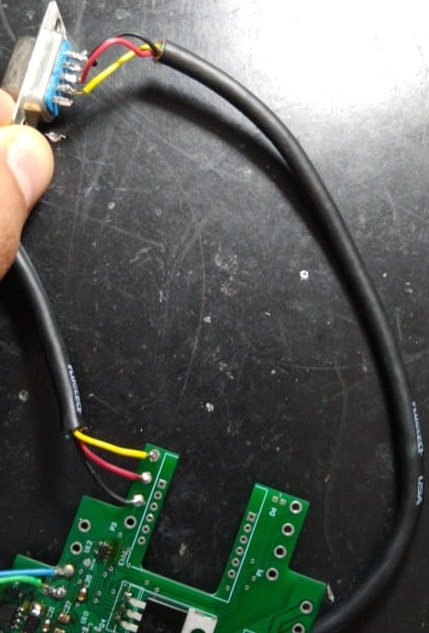
\includegraphics[width=80mm ,keepaspectratio]{Figures/ConRS232.jpeg}
	\caption{ Prueba de la interfaz RS232.}
	\label{fig:Rs232prott}
\end{figure}
La interfaz RS485 fue conectada exitosamente a través de un adaptador de nivel por puerto serie a la computadora, y utilizada durante las pruebas de protocolo Modbus.

Se instaló en el prototipo el módulo wiz820io, de puerto Ethernet, para que en el futuro se pueda programar en el dispositivo una interfaz Ethernet.

%Se establecieron dos salidas diferentes de la placa por las cuales cada una funciona por un estándar diferente. Se adaptaron los niveles de tension para que cada salida fuera capaz de manejar los protocolos deseados.

%\begin{itemize}
%\item Deberá contemplar una posible modificación a futuro para una interfaz ethernet a través de una entrada para rj45.
%\end{itemize}

%Se dejo en el PCB el grabado del footprint de un modulo wiz820io con puerto ethernet y se realizaron los cortes necesarios para que quepa en la carcasa para riel DIN.
 

\subsection{Grupo de requerimientos referidos a diseño del circuito eléctrico}
%\begin{itemize}
%\item El dispositivo deberá poseer como microcontrolador principal MSP430F2418
%\end{itemize}

%Se uso el microcontrolador MSP430F2418 de \textit{texas instrument} con una %referencia de tensión externa y un cristal oscilador de 32768 Hz.

%\begin{itemize}
%\item Se implementaran protecciones contra sobretensión en salida y entradas
%\end{itemize}

%La entrada de alimentación, y la salida de enlace de corriente tienen %protección de sobretensión. 

%\begin{itemize}
%\item Deberá poseer un relé para realizar un corte por corriente.
%\end{itemize}

%Se conecto al microcontrolador un relé para accionarlo según las necesidades.

Se usó el microcontrolador MSP430F2418 de Texas Instruments con una referencia de tensión externa y un cristal oscilador de 32768 Hz. Este puede verse soldado en la placa en la figura \ref{fig:polyrele}.

%\begin{figure}[!htb]
%	\centering
%	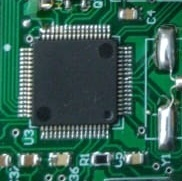
\includegraphics[width=80mm,keepaspectratio]{Figures/miccroenplaca.jpeg}
%	\caption{Microcontrolador soldado.}
%	\label{fig:microenplaca}
%\end{figure}

Un polyswitch que protege a la placa de sobre corriente puede verse en la figura \ref{fig:polyrele} en el sector superior derecha, también puede verse en la misma figura, en la parte inferior derecha, un relé soldado.

\begin{figure}[!htb]
	\centering
	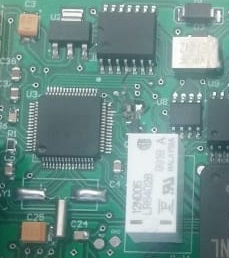
\includegraphics[width=80mm,keepaspectratio]{Figures/polyswitchyrele.jpg}
	\caption{ Area del microcontrolador en el dispositivo.}
	\label{fig:polyrele}
\end{figure}

\subsection{Grupo de requerimientos referidos a diseño  de impresión del circuito}

El diseño de la parte inferior del PCB se realizó teniendo en cuenta que el tipo de soldado fuese por ola de refusión. Los componentes fueron alineados teniendo en cuenta si provocarían sombras de estaño. El diseño puede verse en la figura \ref{fig:PCBbackk}.

%\ref{fig:PCBfrontt}.




 
%\begin{itemize}
%\item Se contempla en el diseño que el tipo de soldado será por refusión por cara superior.

%\item Se contempla en el diseño que el tipo de soldado será por ola en la cara inferior del circuito.
%\end{itemize}

%Ambos requerimientos se cumplieron en la elaboración del prototipo.

%\section{Realización de un manual de usuario}

%Al finalizar las correcciones sobre el software se elaboro un manual de %usuario en un documento online publico donde se especifica el uso del %dispositivo armado, sus partes y conexiones, especificaciones de que %parámetros puede medir y los registros que comunica por protocolo modbus.


%\begin{figure}[!htb]
%	\centering
%	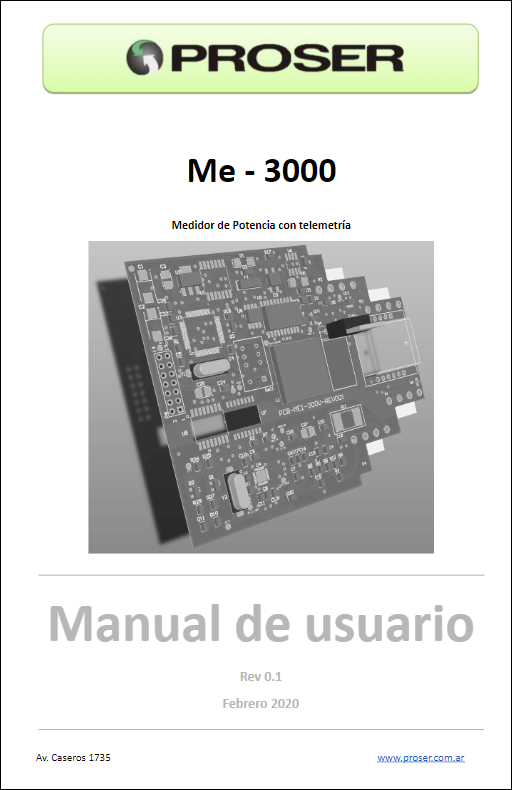
\includegraphics[width=80mm,keepaspectratio]{Figures/portadamanual.png}
%	\caption{Portada del manual elaborado.}
%	\label{fig:ManualPortad}
%\end{figure}

 
% Chapter Template

\chapter{Conclusiones} % Main chapter title

\label{Chapter5} % Change X to a consecutive number; for referencing this chapter elsewhere, use \ref{ChapterX}


%----------------------------------------------------------------------------------------

%----------------------------------------------------------------------------------------
%	SECTION 1
%----------------------------------------------------------------------------------------

\section{Conclusiones generales }
Del trabajo realizado se logró obtener un dispositivo medidor de potencia eléctrica con tolerancias aceptables, capaz de transmitir datos en un entorno industrial.

El trabajo demostró que a partir de requerimientos establecidos por un cliente se puede diseñar la electrónica necesaria para cumplirlos. También se demuestra que el diseño y programación de un prototipo electrónico puede llevarse a cabo de manera completamente remota.

Se cumplieron los requisitos planteados al comienzo del trabajo. Durante la elaboración se encontraron otras necesidades que deberán ser satisfechas en una actualización del software.

Se realizó un manual de usuario para poder comercializar el dispositivo. El manual incluye las limitaciones del dispositivo como también especificaciones de cómo usarlo.

En el desarrollo de este trabajo se aplicaron conocimientos obtenidos de las materias de la Carrera de Especialización en Sistemas Embebidos. Podemos resaltar:

\begin{itemize}
\item Técnicas de ingeniería de software y uso de repositorios para mantener organizadas las versiones tanto del software como del hardware.
\item De la materia \textquotedblleft Diseño de PCB\textquotedblright \  los métodos para nombrar y realizar esquemas prolijos en circuitos de varias hojas.
\item Los fundamentos de la materia \textquotedblleft Diseño para la manufactura electrónica\textquotedblright \  fueron claves para la fabricación del PCB.
\item Los conocimientos de programación y arquitectura de microcontroladores facilitaron la curva de aprendizaje del microcontrolador usado.
\item Los conocimientos de protocolos y comunicaciones digitales al implementar en el software protocolos comúnmente conocidos y protocolos nuevos.
\end{itemize}

%----------------------------------------------------------------------------------------
%	SECTION 2
%----------------------------------------------------------------------------------------
\section{Próximos pasos}

El trabajo elaborado consideraba que en el dispositivo debía implementarse un puerto LAN Ethernet en un futuro. Durante el desarrollo del trabajo se encontraron posibles evoluciones del proyecto. Las siguientes tareas a realizar son:

\begin{itemize}
\item Implementar en el software un driver previamente desarrollado para el puerto LAN Ethernet.
%\item Implementar un menú de calibración del dispositivo para que el fabricante pueda producirlo en masa.
%\item Agregar todos los detalles pertinentes al dispositivo en el manual de usuario. Elaborar la segunda version del manual de usuario.
\item También agregaría valor al trabajo elaborar una aplicación, tipo web app o más compleja, para agregar un método adicional de configurar el dispositivo como también visualizar los datos que este comunica.
\end{itemize}




 

%----------------------------------------------------------------------------------------
%	CONTENIDO DE LA MEMORIA  - APÉNDICES
%----------------------------------------------------------------------------------------

\appendix % indicativo para indicarle a LaTeX los siguientes "capítulos" son apéndices

% Incluir los apéndices de la memoria como archivos separadas desde la carpeta Appendices
% Descomentar las líneas a medida que se escriben los apéndices

%% Appendix A

\chapter{Manual de usuario} % Main appendix title

\label{AppendixA} % For referencing this appendix elsewhere, use \ref{AppendixA}


\section{Descripción}
El medidor (nombre) es un dispositivo capaz de medir tensión y voltaje de línea y realizar cálculos de potencia activa y reactiva, como mediciones de fase. El dispositivo

\section{Características generales}

\begin{itemize}
\item Alimentación de 8 a 28V (AC).
\item Consumo menor a 5700W.
\item Puerto de comunicación serial RS232/Rs485.
\item Menú serie para configuración en boot.
\item Leds de referencia.
\item Capacidad de mediciones alterna para  2200V o 380V.
\end{itemize}


\section{Instalación}

\subsection{Instalación mecánica}

El equipo está diseñado para montaje sobre riel DIN. Se calza sobre riel. EN sus laterales se encuentra una etiqueta con descripción de borneras para el conexionado.


\begin{figure}[!htb]
	\centering
	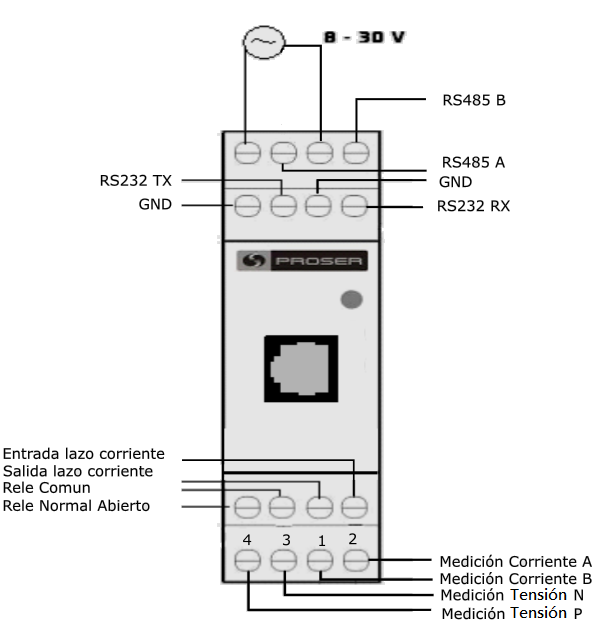
\includegraphics[width=\textwidth , keepaspectratio]{Figures/ApendixA/conectores2.png}
	%\caption{}
	\label{fig:ADEfuncbloc}
\end{figure}

\subsection{Instalación eléctrica }
El equipo se alimenta con tensión continua de un rango de 8 a 40 voltios.
A continuación se detalla la tabla de conexionado:
% Please add the following required packages to your document preamble:
% \usepackage{booktabs}
\begin{table}[!htb]
\begin{tabular}{@{}lll@{}}
\toprule
Borne & REF         & Descripción                \\ \midrule
1     & CloopIO     & Salida lazo corriente 4 20 \\
2     & CloopV      & Entrada 4 20               \\
3     &             & Comun de rele              \\
4     &             & Normal abierto relé        \\
5     & AC          & Entrada alterna medidor    \\
6     & AC          & Entrada alterna medidor    \\
7     & B           & B RS485                    \\
8     & A           & A RS485                    \\
9     & GND digital &                            \\
10    & GND digital &                            \\
11    & RS232 Rx    &                            \\
12    & RS232 Tx    &                            \\
13    & Shunt N     & Medición corriente         \\
14    & Shunt P     & Medición corriente         \\
15    & Voltaje N   & Medición tensión           \\
16    & Voltaje P   & Medición tensión           \\ \bottomrule
\end{tabular}
\end{table}


\subsection{Entradas discretas}

\subsection{Entradas analógicas}

\subsection{Salidas discretas}
El medidor viene provisto de una salida discreta del tipo open collector que puede manejar una carga con una corriente máxima de hasta 100mA.

\subsection{Puerto Serial}
El medidor viene provisto de un puerto de comunicaciones serial que permite conectarse a cualquier dispositivo con puerto RS232 o RS485 .
La velocidad de comunicación  está fijada a 9600bps. Además el puerto se comunica en protocolo Modbus seleccionable de RTU o ASCII con paridad elegible.

\section{Operación}

\subsection{Indicador luminosos LED}

El medidor cuenta con dos indicadores luminosos LED . Un LED indica para la calibración dependiente de la constante de calibración y otro Para indicar el estado del sistema.


El LED del equipo indica:

\begin{itemize}
\item Led (verde) encendido : Corriendo menú serie
\item Led (rojo) encendido: Esperando 10 segundos a menú serie
\item Led (verde) titilante  a 500 ms : Corriendo programa de lectura
\item Led (rojo) titilante  a 500 ms : Puerto 232
\item Led (rojo) apagado : Puerto 485
\item CF2 (Led Q1)  Es proporcional a la potencia activa.
\end{itemize}


\subsection{Configuración}
El medidor tiene embebido un menú, que permite configurar el equipo y realizar pruebas de funcionamiento por medio de un terminal estándar (ej: Hyperterminal de Windows).

Esto permite acceder a la configuración del equipo sin necesidad de un software adicional.

El ingreso al menú de configuración se realiza conectando un terminal configurado en 9600 8N1.


\subsubsection{Menú principal}
En el menú de configuración principal se puede apreciar las opciones de ajuste del equipo.

\textcolor{orange}{
PROSER MEI-380V, S/N: SV-0500003}

\definecolor{mygreen}{RGB}{40, 100, 60}

\textcolor{mygreen}{MenuPrincipal}

\textcolor{blue}{1: Visualización variables.}

\textcolor{blue}{2: Puerto serie.}

\textcolor{blue}{3: Salida 4-20mA.}

\textcolor{blue}{4: Alarma.}

\textcolor{blue}{D: Aplicar valores por defecto globalmente.}

\textcolor{blue}{G: Guarda configuración.}

\textcolor{blue}{ESC: Abandonar terminal.}



Descripción de las Opciones:


\textcolor{blue}{1-2 .}
Ingresando la opción 1 a 4 se accede a las distintas opciones del equipo.

\textcolor{blue}{D .}
Modifica todos los valores a los predeterminados.

\textcolor{blue}{G .}
Guarda la configuración seteada y aplica los cambios.

\textcolor{blue}{ESC.}
Abandona la terminal, esta se cierra hasta que se reinicie el dispositivo.

\subsubsection{OPCIÓN 1: Visualización de variables}
Esta opción permite visualizar las variables que se encuentra recopilando el sensor.

\textcolor{mygreen}{VISUALIZACIÓN DE VARIABLES }

\textcolor{blue}{Tensión (V)}

\textcolor{blue}{Corriente (A)}

\textcolor{blue}{Potencia Activa (W)}

\textcolor{blue}{Potencia Reactiva (W)}

\textcolor{blue}{Frecuencia (Hz)}

\textcolor{blue}{Factor de potencia}

\textcolor{blue}{Totalizado (Kw/h)}

\textcolor{blue}{ESC: Menú principal.}



Descripción de las Opciones

\textcolor{blue}{ESC.}
Abandona este menú, vuelve al menú principal.

\subsubsection{OPCIÓN 2: Puerto serie}

Esta opción configura el puerto serie por lo que se recomienda re-configurar el puerto de comunicación que se esté utilizando al cambiar alguna variable. Esta opción también configura parámetros del protocolo Modbus.

\textcolor{mygreen}{CONFIGURACION PUERTO SERIE}

\textcolor{blue}{1* CONFIGURACION PUERTO SERIE * [Valores predeterminados]}

\textcolor{blue}{1: Baud rate: 9600}

\textcolor{blue}{2: Bits de datos: 8 Bits}

\textcolor{blue}{3: Paridad: NINGUNA}

\textcolor{blue}{4: Bits de parada: 1}

\textcolor{blue}{5: Dirección MODBUS: 5}

\textcolor{blue}{6: Protocolo modo: RTU}

\textcolor{blue}{7: Protocolo tipo: ENRON}

\textcolor{blue}{8: Tipo de puerto: RS485}

\textcolor{blue}{D: Aplica configuración por defecto.}

\textcolor{blue}{ESC: Menú principal.}



Descripción de las Opciones

\textcolor{blue}{1.Baud rate }	
Permite ajustar el Baud Rate del puerto.

\textcolor{blue}{2.Bits de datos}
Ajusta los bits de datos entre 7 u 8 bits.

\textcolor{blue}{3.Paridad}
Ajusta la paridad entre par o impar.

\textcolor{blue}{4.Parada}
Ajusta los bits de parada, puede ser 1 o 2.

\textcolor{blue}{5.Dirección Slave del Modbus}
Setea la dirección de esclavo que tendrá el dispositivo para el protocolo Modbus.

\textcolor{blue}{6.Modo del Protocolo}
Tipo de protocolo MODBUS, puede ser ASCII o RTU.

\textcolor{blue}{8.Tipo de puerto}
Selecciona entre los dos posibles puertos de salida, RS232 o RS485.


\subsubsection{OPCIÓN 3: Salida 4-20mA}
\textcolor{mygreen}{SALIDA ANALOGICA 4-20mA}

\textcolor{blue}{Cambiar variable: Seleccione una opción (1-6)}

\textcolor{blue}{1 - Tensión.}

\textcolor{blue}{2 - Corriente.}

\textcolor{blue}{3 - Potencia Activa.}

\textcolor{blue}{4 - Potencia Reactiva.}

\textcolor{blue}{5 - Frecuencia.}

\textcolor{blue}{6 - Factor de potencia.}

\textcolor{blue}{D: Aplica configuración por defecto.}

\textcolor{blue}{ESC: Menú principal.}


 

Opciones disponibles

\textcolor{blue}{1-6 .}
De estas opciones se elige una variable que se encuentra midiendo el dispositivo. La salida de enlace de corriente es proporcional a la variable elegida.

\textcolor{blue}{D .}
Modifica los valores a los predeterminados.

\textcolor{blue}{ESC.}
Abandona este menú, vuelve al menú principal.

\subsubsection{OPCIÓN 4: Alarma}

Esta opción permite definir qué variable medida será la utilizada para accionar el relé interno y cómo lo accionara.

\textcolor{mygreen}{ALARMA}

\textcolor{blue}{S: Salida a Relé: INACTIVA}

\textcolor{blue}{L1: Límite mínimo para activación: 100}

\textcolor{blue}{L2: Límite máximo para des-activación: 105}

\textcolor{blue}{Cambiar variable: Seleccione una opción (1-6)}

\textcolor{blue}{1 - Tensión.}

\textcolor{blue}{2 - Corriente.}

\textcolor{blue}{3 - Potencia Activa.}

\textcolor{blue}{4 - Potencia Reactiva.}

\textcolor{blue}{5 - Frecuencia.}

\textcolor{blue}{6 - Factor de potencia.}

\textcolor{blue}{Variable asociada: “ ”}

\textcolor{blue}{D: Aplica configuración por defecto.}

\textcolor{blue}{ESC: Menú principal.}

Opciones disponibles


\textcolor{blue}{1-6.}
De estas opciones se elige una variable que se encuentra midiendo el dispositivo. La alarma se activa una vez que el valor de la variable supera el límite de activación.

\textcolor{blue}{D.}
Modifica los valores a los predeterminados.

\textcolor{blue}{ESC.}
Abandona este menú, vuelve al menú principal.




\subsection{TABLA DE REGISTROS MODBUS}

Los registros son solo lectura, en el caso de solicitar un registro que no se encuentre en la tabla se recibirá una excepción.

\begin{table}[h]
%\caption[Registros modbus en software]{Registros generados para la comunicación modbus.}
\begin{tabular}{@{}lllll@{}}
\toprule
\begin{tabular}[c]{@{}l@{}}Dirección \\ del \\ Registro\end{tabular} & \begin{tabular}[c]{@{}l@{}}Número \\ del\\ parámetro\end{tabular} & Descripción                    & Unidades & Tipo de dato \\ \midrule
7001                                                                 & 1                                                                 & Voltaje Instantaneo            & Volts    & Float 32     \\
7003                                                                 & 2                                                                 & Voltaje rms                    & Volts    & Float 32     \\
7005                                                                 & 3                                                                 & Corriente instantánea          & Ampere   & Float 32     \\
7007                                                                 & 4                                                                 & Corriente rms                  & Ampere   & Float 32     \\
7009                                                                 & 5                                                                 & Potencia activa                & Watt     & Float 32     \\
7011                                                                 & 6                                                                 & Potencia reactiva              & VA       & Float 32     \\
7013                                                                 & 7                                                                 & Factor de potencia             & -        & Float 32     \\
7015                                                                 & 8                                                                 & Frecuencia                     & Hz       & Float 32     \\
7017                                                                 & 9                                                                 & Energía reactiva medida        & Joules   & Float 32     \\
7019                                                                 & 10                                                                & Energía activa Total acumulada & kWh      & Float 32    
\end{tabular}
\label{apendixsmodbs}
\end{table}


\subsection{Menú Calibración}
En el menú de configuración principal se puede apreciar las opciones de ajuste del equipo.  
Menú Principal
1: Visualizador de variables
2: Editor de resistencias en uso
3: Editor de registros de ganancia
4: Editor de registros de calibración
5. Editor de salida 4 -20 mA
D: Aplicar valores por defecto globalmente.
G: Guarda configuración.
ESC: Abandonar terminal.

\subsubsection{OPCIÓN 2: Editor de resistencias en uso.}

En esta opción se especifican las resistencias soldadas en el circuito electrónico. Las resistencias que se modifican son las utilizadas para los cálculos de medición.


\textcolor{blue}{2: Editor de resistencias en uso}

Resistores de VP - VN (ohms)

Resistor Shunt (ohms)


\subsubsection{OPCIÓN 3: Editor de registros de ganancia.}
\textcolor{blue}{ Editor de registros de ganancia}

\textcolor{blue}{1 Elija ganancia para PGA\_ IA}

\textcolor{blue}{2 Elija ganancia para PGA\_ V}

Opciones

\textcolor{blue}{1. Ganancia 1  = Fondo de escala 500   mV}

\textcolor{blue}{2. Ganancia 2  = Fondo de escala 250   mV}

\textcolor{blue}{3. Ganancia 4  = Fondo de escala 125   mV}

\textcolor{blue}{4. Ganancia 8  = Fondo de escala 62.5  mV}

\textcolor{blue}{5. Ganancia 16 = Fondo de escala 31.25 mV}

\textcolor{blue}{6. Ganancia 22 = Fondo de escala 22.7  mV}

\subsubsection{OPCIÓN 4: Menú - Calibración de variables:}

Menú - Calibración de variables:

Calibrar Voltaje
\begin{enumerate}
\item Ingreso: Ingrese el voltaje que se está midiendo (cercano al nominal)
\item Se realizan los cálculos
\end{enumerate}

Se ingresa un voltaje cercano al nominal y se realiza el siguiente cálculo

\begin{figure}[!htb]
	\centering
	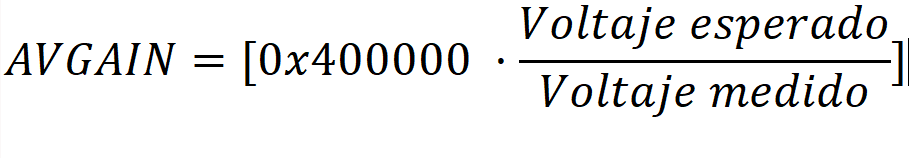
\includegraphics[width=\textwidth , keepaspectratio]{Figures/ApendixA/ec1.png}
	%\caption{}
	\label{fig:ecu1A}
\end{figure}

El resultado se guarda en el registro AVGAIN 


\begin{enumerate}
\setcounter{enumi}{2}
\item Ingreso: Ingrese el voltaje que se está midiendo (menor al 10\% del nominal)
\item Se realizan los cálculos
\end{enumerate}

Se ingresa un voltaje menor al 10\% del nominal y se realiza el siguiente cálculo:

\begin{figure}[!htb]
	\centering
	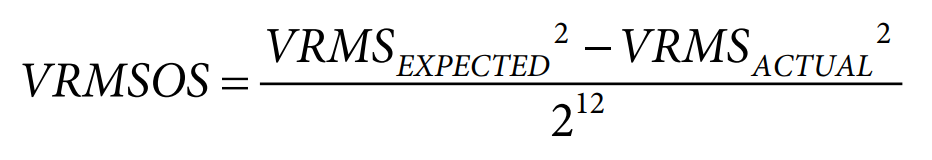
\includegraphics[width=\textwidth , keepaspectratio]{Figures/ApendixA/ec2.png}
	%\caption{}
	\label{fig:ecu2A}
\end{figure}

El resultado se guarda en el registro VRMSOS

\begin{enumerate}
\setcounter{enumi}{4}
\item Se muestra el resultado
\end{enumerate}



Calibrar Corriente

\begin{enumerate}
\item Ingreso: Ingrese la corriente que se está midiendo (cercano al nominal)
\item Se realizan los cálculos
\end{enumerate}

\begin{figure}[!htb]
	\centering
	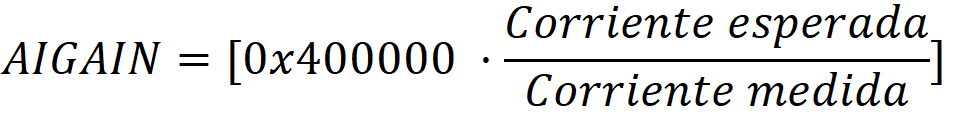
\includegraphics[width=\textwidth , keepaspectratio]{Figures/ApendixA/ec3.png}
	%\caption{}
	\label{fig:ecu3A}
\end{figure}

\begin{enumerate}
\setcounter{enumi}{2}
\item Ingreso: Ingrese la corriente que se está midiendo (menor al 10% del nominal)
\item Se realizan los cálculos
\end{enumerate}
\begin{figure}[!htb]
	\centering
	
\includegraphics[width=\textwidth , keepaspectratio]{Figures/ApendixA/ec4.png}
	%\caption{}
	\label{fig:ecu4A}
\end{figure}

\begin{enumerate}
\setcounter{enumi}{4}
\item Se muestra el resultado
\end{enumerate}

Calibrar Potencia
\begin{enumerate}
\item Ingreso:Se ingresa el valor de la potencia que se está midiendo
\item Se realizan los cálculos
\end{enumerate}

\begin{figure}[!htb]
	\centering
	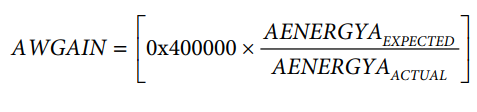
\includegraphics[width=\textwidth , keepaspectratio]{Figures/ApendixA/ec5.png}
	%\caption{}
	\label{fig:ecu5A}
\end{figure}

\begin{enumerate}
\setcounter{enumi}{2}
\item Se muestra el resultado
\end{enumerate}

\subsubsection{OPCIÓN 5: Editor de registros de ganancia}
Menu - Calibración de salida 4-20 mA:
La salida actualmente es dependiente de la variable : “(Se muestra la variable dependiente) ”
Se realizaran 3 mediciones

\begin{itemize}
\item Se inserta el valor mínimo pretendido para 4mA a la placa, se pide que se \item ingrese el valor por consola.
\item Se realizan cálculos.
\item Se Inserta el valor máximo de la variable pretendida para 20mA a la placa, se pide que se ingrese el valor por consola.
\item Se realizan cálculos.
\item Se pide que se inserte un valor intermedio y se pide que ingrese el valor por consola
\item Se calibra y sale del menú

\end{itemize}

%%%%%%%%%%%%%%%%%%%%%%
%%%%%%%%%%%%%%%%%%%%%%%
%%%%%%%%%%%%%%%%%%%%%%%%%

\section{Características técnicas}
Montaje
\begin{itemize}
\item Riel DIN
\end{itemize}
Alimentación
\begin{itemize}
\item 8 a 30 VCC
\item Consumo <0.7W
\end{itemize}
Puertos de comunicación
\begin{itemize}
\item RS232 y RS485 (ambos en el mismo puerto)
\item Bbps: 9600
\item Bits: 8
\item Paridad: Sin paridad.
\item En modo Modbus : RTU/ASCII , Par/ Impar/ Sin paridad.
\end{itemize}
Configuración
\begin{itemize}
\item Menú serie embebido
\end{itemize}
Módulo de medición de potencia
\begin{itemize}
\item Precisión con tolerancia de 1%
\item Registros de medición de potencia reactiva y energía.
\end{itemize}
Entradas /Salidas
\begin{itemize}
\item Una salida de comunicación serie
\item 4 entradas analógicas (2 para medcion de voltaje y 2 para medición de amperaje)
\item 1 salida analógica (4-20MA)
\end{itemize}




\section{Medidas y dimensiones}
\begin{figure}[!htb]
	\centering
	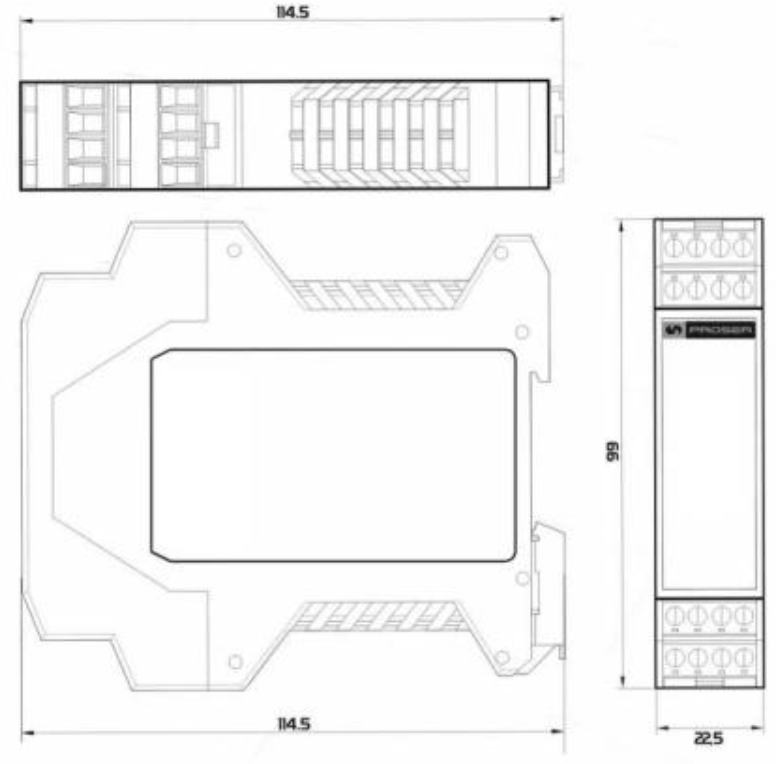
\includegraphics[width=\textwidth , keepaspectratio]{Figures/ApendixA/medidas.png}
	%\caption{}
	\label{fig:ADEfuncbloc}
\end{figure}

Los valores se encuentran en mm  (milímetros).
%% Appendix Template


\chapter{Calibración Medidor} % Main appendix title

\label{AppendixB} % Change X to a consecutive letter; for referencing this appendix elsewhere, use \ref{AppendixX}
\definecolor{mygreen}{RGB}{40, 100, 60}

\section{Menú de Calibración del equipo de medición}


A continuación se muestra el menú de calibración como aparece en el menú serie:

\textcolor{mygreen}{Menú Principal}

\textcolor{blue}{1: Visualizador de variables}

\textcolor{blue}{2: Editor de resistencias en uso}

\textcolor{blue}{3: Editor de registros de ganancia}

\textcolor{blue}{4: Editor de registros de calibración}

\textcolor{blue}{5. Editor de salida 4 -20 mA}

\textcolor{blue}{D: Aplicar valores por defecto globalmente.}

\textcolor{blue}{G: Guarda configuración.}

\textcolor{blue}{ESC: Abandonar terminal.}

\subsection{Opción 2: Editor de resistencias en uso}
Lo primero que se deberá ingresar en el menú son los valores de las resistencias que se encuentran el el dispositivo.

\begin{itemize}
\item En la opción “1.Resistores de VP - VN (kilo ohms)“ inserte el valor del resistor en kilohms, en números enteros, de la resistencia que se encuentra en la parte de medicion de voltaje.

\item En la opción “2.Resistor Shunt (mili ohms)“ se ingresa el valor del resistor shunt en miliohms, en números enteros, del shunt que se encuentra en la medición de corriente.
\end{itemize}


\subsection{Opción 3: Editor de registros de ganancia}

Luego de ingresar los valores de resistencia, el software puede calcular correctamente los parámetros medidos, sin embargo se puede acotar los límites máximos a medir, y definir qué valores se podrán medir modificando los registros de ganancia. Cuanto más alto sea el valor de ganancia que se seleccione más acotado será el rango posible de medición.




Para la opción "Elija ganancia para PGA\_ V":
Se debe elegir la ganancia para la tensión entre las opciones disponibles, es decir seleccionar el valor de  PGA\_ V  que puede ser como mínima una ganancia de 1 y como máximo una ganancia de 16.
Por ejemplo para una resistencia VP -  VN de 990k ohm y una ganancia de PGA\_ V igual a 1 (uno) el dispositivo podra medir como maximo 495Voltios. Por ende el siguiente paso es:

\begin{itemize}
\item En la opción \textquotedblleft Elija ganancia para PGA\_ V\textquotedblright , elija una de las ganancias disponibles.
\end{itemize}

Para la opción \textquotedblleft Elija ganancia para PGA\_ IA\textquotedblright:
Se debe elegir la ganancia para la tensión entre las opciones disponibles, es decir seleccionar el valor de  PGA\_ I  que puede ser como mínima una ganancia de 2 y como máximo una ganancia de 22.
Por ejemplo para una resistencia 0.100 ohm   y una ganancia de PGA\_ IA igual a 1 (uno) el dispositivo podra medir como maximo 2,5A . Por ende el siguiente paso es:

\begin{itemize}
\item En la opción "Elija ganancia para PGA\_ IA” , elija una de las ganancias disponibles.

\end{itemize}

\subsection{Opción 4: Editor de registros de calibración}

Una vez definidas las ganancias, se procede a calibrar las variables dentro del rango mostrado en el menú anterior. Para calibrar el voltaje seleccionamos la primera opción. En esta opción se pedirá que ingrese un valor y se mostrará un número sin unidad, este número es para tener una referencia de que valor aproximado se debe ingresar pues el software siempre comparará la magnitud que se ingresa al hardware y el número que se ingresa en este menú, sin contar con la referencia mostrada. Sin embargo recomiendo seguir la referencia. Entonces:

\begin{itemize}
\item Se ingresa a la opción "1.Calibrar Voltaje”, aquí se debe ingresar numéricamente el valor de voltaje que se inyecte en el puerto de medición VP -VN de la placa, el primer valor debe ser un 10\% del valor máximo admisible por la ganancia del menú previo.
\item Luego se deben ingresar otros 3 valores diferentes, de la misma forma, inyectando al hardware y escribiendo en el software.
\item Finalmente el 5 (quinto) valor a ingresar debería ser uno cercano al valor máximo del rango admisible, se debe inyectar esta magnitud al hardware y escribirla en el software.
\end{itemize}

En este caso donde se editan los registros se pueden utilizar comas al ingresar variables.

Una vez calibrado el voltaje, se puede repetir el paso o avanzar a calibrar la corriente. El menu de calibracion de corriente funciona de igual manera que el de voltaje, si sale del menú en medio del proceso se pierde todo el proceso de calibración y se debe comenzar devuelta, por lo que si se comete un error al ingresar algún dato puede salir para no guardar. Entonces:

\begin{itemize}
\item Se ingresa a la opción "2.Calibrar Corriente", aquí se debe ingresar numéricamente el valor de corriente que se inyecte en el puerto de medición de corriente de la placa, el primer valor debe ser un 10\% del valor máximo admisible por la ganancia del menú previo.

\item Luego se deben ingresar otros 3 valores diferentes, de la misma forma, inyectando al hardware y escribiendo en el software.

\item Finalmente el 5(quinto) valor a ingresar deberia ser uno cercano al valor máximo del rango admisible, se debe inyectar esta magnitud al hardware y escribirla en el software.
\end{itemize}

La siguiente variable a calibrar es la potencia,  aunque probablemente con calibrar las variables anteriores sea suficiente. Entonces el siguiente paso:

\begin{itemize}
\item Se ingresa a la opción "3.Calibrar Potencia", aquí se debe ingresar numéricamente el valor de potencia activa que debería poder medirse, se debe ingresar diversos valores cinco veces.
\end{itemize}

\subsection{Opción 5: Menu - Calibración de salida 4-20 mA}

En este menú se puede editar los puntos de salida del enlace de corriente 4-20mA de manera manual. Se selecciona el punto de salida, ya sea el límite inferior 4mA o el superior 20mA , y luego se puede aumentar o disminuir la corriente para que la salida coincida verdaderamente con el valor esperado.

En la parte "1. Ajustar puntos salida de corriente":

\begin{itemize}
\item En "1. Ajustar puntos salida de corriente" , selecciona  “1.  Ajustar salida a 4 mA” de aquí se debe medir la salida analogica con un instrumento de medición secundario y luego hacer variar la magnitud con las opciones disponibles hasta que coincida con los 4 miliamperes correspondientes.

\item En "1. Ajustar puntos salida de corriente" , selecciona  “2. Ajustar salida a 20 mA” de aquí se debe medir la salida analogica con un instrumento de medición secundario y luego hacer variar la magnitud con las opciones disponibles hasta que coincida con los 20 miliamperes correspondientes.
Después de calibrar la salida se puede verificar que los valores sean adecuados en la opción “2. Verificar puntos salida de corriente”

\item En  la opción "2. Verificar puntos salida de corriente" se ingresa en cada etapa el valor medido . Al ingresar todos los valores se muestra el error de la salida para 4 mA, 12 mA y 20 mA.
\end{itemize}



\section{Resumen}
%Ecos del grado  \textdegree .
 
2: Editor de resistencias en uso
\begin{enumerate}
\item En la opción “1.Resistores de VP - VN (kilo ohms)“ inserte el valor del resistor en kilohms, en números enteros, de la resistencia que se encuentra en la parte de medicion de voltaje.
\item En la opción “2.Resistor Shunt (mili ohms)“ se ingresa el valor del resistor shunt en miliohms, en números enteros, del shunt que se encuentra en la medición de corriente.
\end{enumerate}


3: Editor de registros de ganancia
\begin{enumerate}
\setcounter{enumi}{2}
\item En la opción \textquotedblleft Elija ganancia para PGA\_ V\textquotedblright , elija una de las ganancias disponibles.
\item En la opción \textquotedblleft Elija ganancia para PGA\_ IA\textquotedblright , elija una de las ganancias disponibles.
\end{enumerate}


4: Editor de registros de calibración
\begin{enumerate}
\setcounter{enumi}{4}
\item Se ingresa a la opción ""1.Calibrar Voltaje”, aquí se debe ingresar numéricamente el valor de voltaje que se inyecte en el puerto de medición VP -VN de la placa, el primer valor debe ser un 10% del valor máximo admisible por la ganancia del menú previo.
\item Luego se deben ingresar otros 3 valores diferentes, de la misma forma, inyectando al hardware y escribiendo en el software.
\item Finalmente el 5 (quinto) valor a ingresar deberia ser uno cercano al valor máximo del rango admisible, se debe inyectar esta magnitud al hardware y escribirla en el software.
\item Se ingresa a la opción "2.Calibrar Corriente", aquí se debe ingresar numéricamente el valor de corriente que se inyecte en el puerto de medición de corriente de la placa, el primer valor debe ser un 10% del valor máximo admisible por la ganancia del menú previo.
\item Luego se deben ingresar otros 3 valores diferentes, de la misma forma, inyectando al hardware y escribiendo en el software.
\item Finalmente el 5 (quinto) valor a ingresar deberia ser uno cercano al valor máximo del rango admisible, se debe inyectar esta magnitud al hardware y escribirla en el software.
\item Se ingresa a la opción "3.Calibrar Potencia", aquí se debe ingresar numéricamente el valor de potencia activa que debería poder medirse, se debe ingresar diversos valores cinco veces.
\end{enumerate}


5: Menu - Calibración de salida 4-20 mA
\begin{enumerate}
\setcounter{enumi}{11}
\item En "1. Ajustar puntos salida de corriente" , selecciona  “1.  Ajustar salida a 4 mA” de aquí se debe medir la salida analogica con un instrumento de medición secundario y luego hacer variar la magnitud con las opciones disponibles hasta que coincida con los 4 miliamperes correspondientes.
\item En "1. Ajustar puntos salida de corriente" , selecciona  “2. Ajustar salida a 20 mA” de aquí se debe medir la salida analogica con un instrumento de medición secundario y luego hacer variar la magnitud con las opciones disponibles hasta que coincida con los 20 miliamperes correspondientes.
\item En  la opción "2. Verificar puntos salida de corriente" se ingresa en cada etapa el valor medido . Al ingresar todos los valores se muestra el error de la salida para 4 mA, 12 mA y 20 mA.
\end{enumerate}




%\include{Appendices/AppendixC}

%----------------------------------------------------------------------------------------
%	BIBLIOGRAPHY
%----------------------------------------------------------------------------------------

\Urlmuskip=0mu plus 1mu\relax
\raggedright
\printbibliography[heading=bibintoc]

%----------------------------------------------------------------------------------------

\end{document}  
